\documentclass[12pt]{report}

% package to activate greek language 
\usepackage[greek,english]{babel}
\usepackage{indentfirst}

% DOCUMENT LAYOUT
\usepackage{geometry} 
\geometry{a4paper, textwidth=5.5in, textheight=8.5in, marginparsep=7pt, marginparwidth=.6in}
\setlength\parindent{8mm}
\setlength\parskip{5mm}

% FONTS
\usepackage{xltxtra}
\usepackage[table]{xcolor}
\defaultfontfeatures{Mapping=tex-text}
\usepackage{libertine}


% package to handle graphics
\usepackage{graphicx}
% package to handle multiple figures in a minipage
\usepackage{subfigure}
%package to activate XeTeX font manager
\usepackage{fontspec}


% MATH
\usepackage{amsmath}

% PDF SETUP
% ---- FILL IN HERE THE DOC TITLE AND AUTHOR
\usepackage[driverfallback=dvipdfmx, bookmarks, colorlinks, breaklinks, pdftitle={Efi Kaltirimidou},pdfauthor={efikalti}]{hyperref}  
\hypersetup{linkcolor=blue,citecolor=blue,filecolor=black,urlcolor=blue} 

% change captions especially for greek language - if the document is in ENGLISH, they should vanish
\addto\captionsenglish{%
  \renewcommand\prefacename{Πρόλογος}%
  \renewcommand\refname{Αναφορές}%
  \renewcommand\abstractname{Περίληψη}%
  \renewcommand\bibname{Βιβλιογραφία}%
  \renewcommand\chaptername{Κεφάλαιο}%
  \renewcommand\appendixname{Παράρτημα}%
  \renewcommand\contentsname{Περιεχόμενα}%
  \renewcommand\listfigurename{Κατάλογος Σχημάτων}%
  \renewcommand\listtablename{Κατάλογος Πινάκων}%
  \renewcommand\indexname{Ευρετήριο}%
  \renewcommand\figurename{Σχήμα}%
  \renewcommand\tablename{Πίνακας}%
  \renewcommand\partname{Μέρος}%
  \renewcommand\enclname{Συνημμένα}%
  \renewcommand\ccname{Κοινοποίηση}%
  \renewcommand\headtoname{Προς}%
  \renewcommand\pagename{Σελίδα}%
  \renewcommand\seename{βλέπε}%
  \renewcommand\alsoname{βλέπε επίσης}%
  \renewcommand\proofname{Απόδειξη}%
  }

%%%%%%%%% END OF PREAMBLE %%%%%%%%%%%%

\begin{document}

% make title out of \author, \title, \date  specified in the preamble
\begin{titlepage}
%
%
\begin{figure}[ht]
\begin{minipage}{0.15\textwidth}
\vspace{-10mm}

\includegraphics[width=20mm]{../images/aristotle_logo.png}
\end{minipage}
%
\begin{minipage}{0.70\textwidth}
{
ΑΡΙΣΤΟΤΕΛΕΙΟ ΠΑΝΕΠΙΣΤΗΜΙΟ\\[0.5\baselineskip]
ΘΕΣΣΑΛΟΝΙΚΗΣ\\[0.5\baselineskip]
Πρόγραμμα Μεταπτυχιακών Σπουδών\\[0.5\baselineskip]
Τεχνητής Νοημοσύνης
}
\end{minipage}
%
\end{figure}

\vspace{10mm}
\hbox{ % Horizontal box
\hspace*{0.08\textwidth} % Whitespace to the left of the title page
\rule{1.5pt}{0.80\textheight} % Vertical line
\hspace*{0.02\textwidth} % Whitespace between the vertical line and title page text
\parbox[b]{0.90\textwidth}{ % Paragraph box which restricts text to less than the width of the page


{\large \textsc{Πτυχιακή Εργασία}}\\[\baselineskip] % Tagline or further description
{\noindent\LARGE\bfseries
Δημιουργία περιεχομένου για Video Games με μεθόδους Procedural Content Generation και Generative Adversarial Neural Networks.
}\\[2\baselineskip] % Title

{\Large Ευφροσύνη Καλτιριμίδου}\\[3\baselineskip] % Author name

{\em Επιβλέπων:}\\[0.25\baselineskip]
{\large Νίκος Νικολαίδης}\\[0.25\baselineskip]
{\large Καθηγητής}

\vspace{0.15\textheight} % Whitespace between the title block and the publisher
{\noindent Θεσσαλονίκη 2020}\\[\baselineskip] % Publisher and logo
}}
%
%
\end{titlepage}

%\newpage
\thispagestyle{empty}
\phantom{~}
\vfill

% Create table of contents
\tableofcontents
%\newpage
\thispagestyle{empty}
\phantom{~}
\vfill

% Intro
\chapter{Εισαγωγή}

\par
Το αντικείμενο της δημιουργίας περιεχομένου(Content Generation) είναι ένα πεδίο της Τεχνητής Νοημοσύνης με εφαρμογές στην ανάπτυξη ηλεκτρονικών παιχνιδιών, στην μουσική, στις ταινίες και σε πολλούς ακόμα τομείς. Μπορούμε να διακρίνουμε δύο διαφορετικές κατηγορίες δημιουργίας περιεχομένου με βάση τα είδη των αλγορίθμων που εφαρμόζονται σε κάθε κατηγορία. Αυτή η εργασία ερευνά τις δύο αυτές κατηγορίες και την αλληλεπίδραση που μπορεί να δημιουργηθεί μεταξύ τους.
\par
Η πρώτη κατηγορία αφορά τη δημιουργία περιεχομένου με τη χρήση ντετερμινιστικών αλγορίθμων (Procedural Content Generation), και η δεύτερη κατηγορία περιέχει την δημιουργία περιεχομένου με την χρήση μηχανικής μάθησης (Machine Learning). Η μέθοδος του Procedural Content Generation (PCG), είναι η παλαιότερη από τις δύο και αυτή με τις περισσότερες εφαρμογές και ερευνητικό περιεχόμενο. Η μέθοδος του Machine Learning (ML) έχει γνωρίσει μεγάλη ανάπτυξη τα τελευταία χρόνια και αποδίδει εντυπωσιακά αποτελέσματα όπου εφαρμόζεται με σωστή έρευνα και ανάπτυξη.

\section{Στόχοι της εργασίας}
\par
Ο βασικός στόχος αυτής της εργασίας είναι η ανάπτυξη δύο συστημάτων παραγωγής δισδιάστατων επιπέδων παιχνιδιού με μια συγκεκριμένη διάταξη. Εφαρμόστηκαν αλγόριθμοι και από τις δύο κατηγορίες για την δημιουργία ενός απλού δισδιάστατου (2D) επιπέδου. Το επίπεδο έχει πολλά κοινά με πραγματικά επίπεδα όπως αυτά αναπαρίστανται σε 2D ηλεκτρονικά παιχνίδια. Περιέχει δωμάτια, διαδρόμους και τοίχους, με μια συγκεκριμένη διάταξη στον διαθέσιμο χώρο του επιπέδου.
\par
Αρχικός στόχος είναι η ανάπτυξη ενός PCG συστήματος παραγωγής επιπέδων με την διάταξη που έχουμε ορίσει. Τα επίπεδα πρέπει να είναι διαφορετικά το ένα από το άλλο όσο περισσότερο γίνεται χωρίς όμως να έχουν διαφορετική διάταξη. Το σύστημα πρέπει να μπορεί να παράγει και να αποθηκεύει με μια συγκεκριμένη μορφή, πολλά επίπεδα σε μικρό χρονικό διάστημα. Το PCG σύστημα είναι ο δημιουργός του συνόλου δεδομένων εκπαίδευσης που θα χρησιμοποιηθεί στο ML σύστημα.
\par
Τελικός στόχος της εργασίας είναι η ανάπτυξη ενός ML συστήματος, και συγκεκριμένα ενός Generative Adversarial Network (GAN), συστήματος, το οποίο θα μπορεί να διαβάζει τα επίπεδα που δημιουργήθηκαν από τον PCG σύστημα και να εκπαιδεύεται από αυτά ώστε να μπορεί να παράγει αντίστοιχα μόλις του ζητηθεί.
\par
Αν και η αναπαράσταση των επιπέδων κρατήθηκε πολύ απλή, υπάρχουν πολλές δυσκολίες που πρέπει να επιλυθούν και για τις δύο κατηγορίες ώστε να παραχθούν ικανοποιητικά αποτελέσματα.

\section{Προκλήσεις και δυσκολίες}
\par
Η μεγαλύτερη πρόκληση που αντιμετωπίστηκε κατά την ανάπτυξη αυτής της εργασίας ήταν η σχεδίαση της αρχιτεκτονικής που θα έχει το μοντέλο του GAN στο ML σύστημα. Το GAN είναι ένα είδος νευρωνικού δικτύου, και η αρχιτεκτονική του αφορά το είδος, την ιεραρχία και τις παραμέτρους των επιπέδων που το αποτελούν. Η αρχιτεκτονική του νευρωνικού δικτύου αλλάζει ραγδαία ανάλογα με το είδος της εφαρμογής στην οποία θα εφαρμοστεί. Για αυτού του είδος τις εφαρμογές, \textit{ανάπτυξη περιεχομένου}, δεν υπάρχουν πολλές υλοποιήσεις διαθέσιμες, ειδικά με τα κριτήρια που απαιτούνται στο συγκεκριμένο πρόβλημα. Συνεπώς η αρχιτεκτονική του δικτύου βρέθηκε μετά από πολλές δοκιμές και πειραματισμούς.
\par
Όπως αναφέρθηκε, η κατηγορία της δημιουργία περιεχομένου με την χρήση μηχανικής μάθησης είναι πολύ πιο πρόσφατη και λιγότερο διαδεδομένη από την κατηγορία του PCG. Συνεπώς έχει λιγότερα παραδείγματα και βιβλιογραφία από την οποία μπορούμε να πάρουμε ιδέες και λύσεις. Αυτή η δυσκολία είναι που την κάνει και πιο ενδιαφέρουσα.
\par
Μια ακόμα δυσκολία που αντιμετωπίστηκε ήταν η μεταφορά των επιπέδων μεταξύ συστημάτων. Τα δύο συστήματα, PCG και ML, είναι ανεπτυγμένα σε διαφορετικές γλώσσες προγραμματισμού το καθένα, έχουν διαφορετικά είδη δεδομένων και έπρεπε να μπορούν να διαβάζουν και να αποθηκεύουν τα επίπεδα με μια κοινή μορφή. Αυτό είχε μια επιπλέον δυσκολία για το ML σύστημα καθώς τα δεδομένα πρέπει να περάσουν από ένα στάδιο προ επεξεργασίας, το οποίο τα αλλοιώνει, συνεπώς πριν την αποθήκευση τους από το ML σύστημα έπρεπε να περάσουν από την αντίστοιχη προ επεξεργασία με την αντίθετη μετατροπή για να είναι αναγνώσιμα από το σύστημα PCG.


\section{Περιεχόμενα}
Στο κεφάλαιο 2 γίνεται μια περιγραφή της θεωρίας και εννοιολογίας του PCG καθώς και μερικών από των πιο αντιπροσωπευτικών αλγορίθμων. Στο κεφάλαιο 3 αναλύεται πως υλοποιήθηκε το σύστημα PCG σε αυτή την εργασία, σε αναφορά και με το προηγούμενο κεφάλαιο. Με την ίδια λογική, στο κεφάλαιο 4 γίνετε μια θεωρητική ανάλυση του τομέα του ML, με έμφαση στις μεθόδους που χρησιμοποιήθηκαν στην υλοποίηση η οποία αναλύεται στο κεφάλαιο 5 μαζί με τα αποτελέσματα που παρήχθησαν από την εκπαίδευση του συστήματος ML. Στο προτελευταίο κεφάλαιο, 6, αναλύουμε τα συμπεράσματα που προέκυψαν από αυτή την εργασία και μελλοντικές προτάσεις. Το τελευταίο κεφάλαιο, 7, περιέχει αναφορές στην βιβλιογραφία και συνδέσμους σε πηγές για την θεωρητική και τεχνική τεκμηρίωση της εργασίας.






% Procedural Content Generation
% print no page number
\thispagestyle{empty}

\chapter{Procedural Content Generation}

Το αντικείμενο του Procedural Content Generation (PCG) όπως ορίζεται στο 
\cite{pcgdef} είναι η \textit{Δημιουργία περιεχομένου για ηλεκτρονικά παιχνίδια με την χρήση αλγορίθμων και με την παροχή ελάχιστων ή καθόλου εισόδων από τον χρήστη}. Αποτελεί μια μεγάλη κατηγορία έρευνας και ανάπτυξης τόσο στην βιομηχανία των  παιχνιδιών όσο και στην επιστήμη της πληροφορικής \cite{futureofcontent}.
\par
Το PCG, όπως και πολλά άλλα αντικείμενα της πληροφορικής, αντιπροσωπεύεται από ιδιαίτερα προβλήματα και περιορισμούς τόσο στην πολυπλοκότητα των αλγορίθμων όσο και στην αυθεντικότητα και προτοτυπία των αποτελεσμάτων.  Ως γνωστικό αντικείμενο της επιστήμης της πληροφορικής, μπορεί να ταξινομηθεί κάτω από την κατηγορία της Τεχνητής Νοημοσύνης καθώς βασικός στόχος του PCG είναι η δημιουργία αλγορίθμων που μπορούν να προσομοιώσουν την ανθρώπινη δημιουργικότητα και ευφυία. Επιπλέον στα προβλήματα και στις προσεγγίσεις επίλυσης παρατηρούμε πολλά κοινά με άλλα πεδία της Τεχνητής Νοημοσύνης.
\par
Όπως έχει παρατηρηθεί και σε πολλά άλλα αντικείμενα της Τεχνητής Νοημοσύνης, έτσι και το PCG είχε μικρή εξάπλωση και χρήση στην αρχή. Αυτό δεν οφείλεται στις δυνατότητες των αλγορίθμων και στην θεωρία πίσω από το αντικείμενο, αλλά κυρίως στην αδυναμία του υλικού (hardware) των υπολογιστών εκείνων των περιόδων να χρησιμοποιήσουν αλγόριθμους τέτοιας πολυπλοκότητας. Τα τελευταία χρόνια με την ανάπτυξη των δυνατοτήτων των προσωπικών υπολογιστών και των κινητών συσκευών έχει διευρυνθεί η χρήση μεθόδων PCG για την παραγωγή διαφόρων ειδών game content όπως θα αναλυθεί στη συνέχεια. Μαζί με την αύξηση στην χρήση μεθόδων PCG ήρθε και η αύξηση των προβλημάτων που καλείται να επιλύσει.

\begin{figure}[ht]
\centering
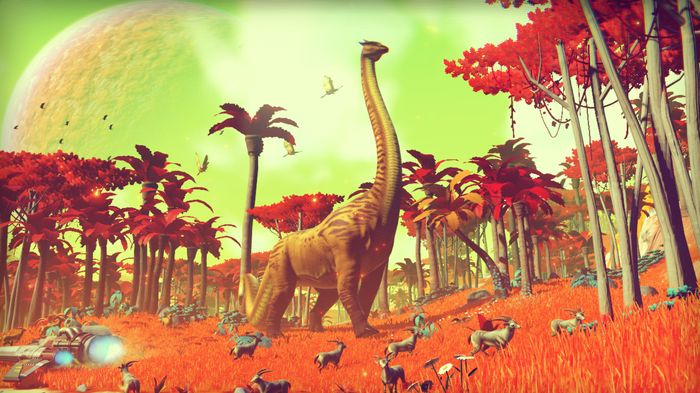
\includegraphics[width=4in]{../images/no-mans-sky.jpg}
\caption{Screenshot από το παιχνίδι No Man's Sky (2016). Οι κόσμοι που δημιουργεί είναι εξ'ολοκλήρου κατασκευασμένοι με τη χρήση ντετερμινιστικών μεθόδων Procedural Content Generation.}
\end{figure}

\section{Περιεχόμενο}
Για να κατανοήσουμε καλύτερη το πεδίο του PCG πρέπει πρώτα να καταλάβουμε τι θεωρείται περιεχόμενο (Game Content) σε ένα παιχνίδι. Ο τομέας του PCG αναφέρεται και έχει χρησιμοποιηθεί σε ηλεκτρονικά παιχνίδια (Video Games), επιτραπέζια παιχνίδια (Board Games), παιχνίδια με κάρτες (Card Games) κ.ά. Το αντικείμενο της συγκεκριμένης εργασίας, επικεντρώνετε στην δημιουργία περιεχομένου για Video Games.

\begin{description}
\item [Game Content] Όπως αναφέρεται και στο όνομα, περιεχόμενο, είναι κάτι που περιέχεται σε ένα παιχνίδι. Αυτός ο ορισμός όμως είναι πολύ γενικός και ευρύς και δεν περιορίζετε μόνο στο περιεχόμενο που αντιστοιχεί στο PCG. Στην βιβλιογραφία μπορούμε να ξεχωρίσουμε συγκεκριμένα είδη περιεχομένου \cite{typesofcontent} που φαίνετε να μπορούν να δημιουργηθούν με μεθόδους PCG. Αυτά είναι:
\end{description}

\begin{itemize}
  \item Γραφικά (Textures)
  \item Επίπεδα (Levels) και χάρτες (Maps)
   \item Αντικείμενα (Items)
   \item Αποστολές (Quests)
   \item Ιστορίες (Stories)
   \item Μουσική (Music)
\end{itemize}

Ο παραπάνω διαχορισμός γίνεται με βάση το είδος του κάθε περιεχομένου, για παράδειγμα η μουσική ως περιεχόμενο ενός παιχνιδιού, διαφέρει από τα αντικείμενα. Αντίστοιχα οι μεθοδολογίες που έχουν αναπτυχθεί για την παραγωγή μουσικής διαφέρουν από τις μεθόδους που χρησιμοποιούνται για την παραγωγή αντικειμένων. Αυτό βέβαια δεν σημαίνει ότι δεν υπάρχουν κοινοί αργόριθμοι που μπορούν να εφαμροστούν σε παραπάνω από ένα είδος με επιτυχία, αντίθετα υπάρχουν πολλοί αλγόριθμοι που έχουν ως βάση έναν πιο γενικό αλγόριθμο και αποτελούν ειδικές εκδόσεις του για το κάθε είδος περιεχομένου.
\par
Ο διαχωρισμός του περιεχομένου βοηθάει στην καλύτερη κατανόηση των ιδιαιτεροτήτων και των περιορισμών που εμφανίζει το κάθε είδος το οποίο οδηγεί στην δημιουργία καλύτερων μεθόδων και αλγορίθμων.

\section{Η χρησιμότητα του PCG}
	Η πρώτη ανάγκη που παρουσιάστηκε και οδήγησε στην υιοθέτηση μεθόδων PCG αφορούσε την μείωση του αποθηκευτικού χώρου που καταλάμβανε ένα παιχνίδι. Το PCG δίνει την δυνατότητα τις δημιουργίας content μόλις παρουσιαστεί η ανάγκη να χρησιμοποιηθεί ή να παρουσιαστεί στον παίκτη, το οποίο σημαίνει ότι δεν χρειάζετε να καταλαμβάνει χώρο στην μνήμη εάν υπάρχει η δυνατότητα δημιουργίας του ακριβώς την στιγμή που χρειάζεται. Με την μνήμη να αποτελεί έναν διαμοιραζόμενο πώρο μεταξύ των εφαμρογών ακόμα και σήμερα το PCG αποτελεί μια μέθοδο μείωσης του χώρου που καταλαμβάνει ένα παιχνίδι.
\par
	Το PCG έχει επίσης χρησιμότητα από τους καλλιτέχνες και σχεδιαστές διαφόρων παιχνιδιών. Η χρήση PCG για την δημιουργία περιεχομένου το οποίο αν και δεν είναι τέλειο ή αρκετά καλό για το παιχνίδι, δίνετε στους σχεδιαστές οι οποίοι το βελτιώνουν, το αλλάζουν και προσθέτουν στοιχεία ώστε προστεθεί με επιτυχία στο παιχνίδι. Με αυτόν τον τρόπο το PCG βοηθάει τους ανθρώπους με τέτοιους ρόλους στην εργασία τους, δίνοντας του έμπνευση και κάνοντας ένα κομμάτι της δουλειάς ώστε αυτοί να μπορούν να δώσουν προσοχή στις λεπτομέρειες που θα κάνουν το περιεχόμενο πραγματατικά εντυπωσιακό. Σε αυτές τις υλοποιήσεις του PCG συνηθίζεται να δίνει ο σχεδιαστής μέσω διαφόρων εισόδων κάποιες παραμέτρους που ορίζουν μια γενική περιγραφή του περιεχομένου που θέλει να δημιουργήσει, για παράδειγμα το μέγεθος του χάρτη ή το είδος των πόρων που θα έχει διαθέσιμα. Στη συνέχεια το PCG δημιουργεί το περιεχόμενα με βάση τις παραμέτρους που πήρε και εμφανίζει το αποτέλεσμα στο σχεδιαστή. Αυτή η διαδικασία μπορεί να επαναληφθεί πολλές φορές μέχρι να δημιουργεί το επιθυμητό αποτέλεσμα.
\par
	Μια επίσης πολύ σημαντική ανάγκη που καλύπτει, εν μέρη, το PCG είναι η δημιουργία ενός παιχνιδιού που δεν τελειώνει ποτέ. Αντίθετα με την συνεχή παραγωγή πρωτότυπου και ποικίλου περιεχομένου, ένα παιχνίδι μπορεί να συνεχίζετε επ άπειρον, προσφέροντας αμέτρητες ώρες gameplay στους παίκτες. Πολλά παιχνίδια έχουν επιχειρήσει να υλοποιήσουν αυτό το feauture, κάποια με μεγάλη επιτυχία και κάποια με το αντίθετο αποτέλεσμα. Ένα από τα μεγαλύτερα προβλήματα που αντιμετωπίζουν οι υλοποιήσεις του PCG είναι η επαναληψιμότητα και η μονοτονία, όπως θα αναλυθεί και παρακάτω. Είναι ένα από τα πιο σημαντικά κριτήρια για την επιτυχία ενός endless παιχνιδιού.
\par
	Τέλος, μια ανάγκη που έχει προκύψει τα τελευταία χρόνια στον χώρο των παιχνιδιών και συνδέετε με μια ακόμα περιοχή της Τεχνητής Νοημοσύνης στα παιχνίδια είναι η εξατομίκευση περιεχομένου, ή personalized content. Αναφέρεται στην δημιουργία περιεχομένου που είναι σχεδιασμένο για τις προτιμήσεις και τις ανάγκες του κάθε παίκτη.

\section{Παιχνίδια που χρησιμοποιούν PCG}

Από την πρώτη στιγμή που ξεκίνησε η διάδωση των Video Games φάνηκε η ανάγκη για την αυτόματη και αυτόνομη δημιουργία   \textit{σωστού} περιεχομένου. Κάποια από τα παιχνίδια που εφάρμοσαν με μεγάλη επιτυχία μεθόδους PCG είναι:

\begin{description}
\item [Rogue (\textbf{1980})] Ένα από τα πρώτα παιχνίδια που εφάρμοσε PCG για την αυτόματη δημιουργία επιπέδων (\textbf{levels}). To Rogue ενέπνευσε την δημιουργία πολλών παιχνιδιών με αντίστοιχες δυνατότητες και PCG μεθόδους.

\item [Spore (\textbf{2008})] To Spore είναι ένα life-simulation και strategy παιχνίδι που χρησιμοποιεί PCG για την δημιουργία πλασμάτων και αντικειμένων. Οι αλγόριθμοι του Spore, συνδυάζουν απλά σχήματα και αντικείμενα για να δημιουργήσουν μεγαλύτερα και πιο πολύπλοκα πλάσματα με βάση διάφορους κανόνες και περιορισμούς. 

\item [No Man's Sky (\textbf{2016})] Ένα από τα πιο σημαντικά παραδείγματα για τις δυνατότητες του PCG είναι το παιχνίδι no Man's Sky. Το θέμα του παιχνιδιού είναι η εξερεύνηση του διαστήματος και η επιβίωση σε ξένους πλανήτες. Το παιχνίδι δημιουργεί σχεδόν όλόκληρο τον κόσμο με PCG, δηλαδή τους πλανήτες, τα αστέρια, τα φυτά, τα ζώα και τα encounters του παίκτη με τη χρήση ντετερμινιστικών αλγορίθμων PCG. Η αποδοχή του παιχνιδιού από το κοινό ήταν μέτρια. Οι δημιουργοί είχαν υποσχεθεί έναν απέραντο κόσμο γεμάτο περιεχόμενο και οι παίκτες παρατήρησαν ότι το τελικό αποτέλεσμα ήταν μονότονο και επαναλαμβανόμενο, κάτι που τους δημιούργησε άσχημες εντυπώσεις. 
\end{description}

\section{Προβλήματα του PCG}
Όπως αναφέρθηκε και παραπάνω, το PCG δεν αποτελεία μια τέλεια και ολοκληρωμένη λύση για να τα προβλήματα που καλείται να αντιμετωπίσει. Αντίθετα οι υλοποιήσεις του PCG πρέπει να λαμβάνουν υπόψη τα καινούργια προβλήματα και περιορισμούς που δημιουργούνται με την χρήση PCG αλγορίθμων. 

\begin{description}
\item [Επαναληψιμότητα - Μονοτονία] Ένα από τα πιο σημαντικά θέματα είναι η ποικιλία και μοναδικότητα του παραγόμενου περιεχομένου. Όπως αναλύθηκε και παραπάνω, σε πολλές περιπτώσεις το παραγόμενο περιεχόμενο είναι πολύ μονότονο, μοτίβα φαίνονται να επαναλαμβάνονται και κατά συνέπεια το αποτέλεσμα δίνει στον χρήστη την αντίθετη εντύπωση από την επιθυμητή. Οι λόγοι που συμβαίνει αυτό είναι πολλοί και σχετίζονται με το είδος του αλγόριθμου που χρησιμοποιείται κάθε φορά, τις παραμέτρους που δίνονται και τα βασικά assets που χρησιμοποιεί για να δημιουργήσει το περιεχόμενο. 

\item [Ταχύτητα - πολυπλοκότητα] Πολλοί αλγόριθμοι PCG πρέπει να είναι σε θέση να λειτουργούν σε πολύ λίγο χρόνο και με περιορισμένους πόρους. Σε ένα ηλεκτρονικό παιχνίδι υπάρχουν πολλά κομμάτια που πρέπει να δουλεύουν ταυτόχρονα, όπως τα γραφικά, το UI, το σύστημα κανόνων για την προσομοίωση της φυσικής στον κόσμο του παιχνιδιού κ.ά. Συνεπώς το σύστημα του AI που περιέχει και το PCG δεν μπορεί να καταλαμβάνει πολλούς πόρους ή να αργεί να ανταποκριθεί γιατί το παιχνίδι θα φαίνετε να κολλάει ή να μην δουλεύει όπως πρέπει. Αυτό σημαίνει ότι οι αλγόριθμοι που υλοποιούν το PCG πρέπει να έχουν συγκεκριμένη χρονική και χωρική πολύπλοκότητα και να μην ξεπερνάνε.

\item [Playability] Μπορεί να έχουμε σχεδιάσει τον τέλειο αλγόριθμο PCG που χρησιμοποιεί ελάχιστους πόρους του συστήματος και δημιουργεί μοναδικά επίπεδα για το 2D platformer παιχνίδι μας αλλά ένα στα τρία επίπεδα να μην έχουν είσοδο.Αυτό σημαίνει ότι ο παίκτης δεν θα μπορέσει να το επισκεφτεί ποτέ, ή θα βρεθεί παγιδευμένος μέσα του χωρίς κάποιο τρόπο να προχωρήσει το παιχνίδι. Αυτό φυσικά είναι κάτι που δεν θέλουμε σε καμία περίπτωση να συμβεί. Για αυτό το λόγο πρέπει να ορίσουμε τι θεωρείται "playable" περιεχόμενο και τι "unplayable".
 
\end{description}


\section{Επιθυμητά Χαρακτηριστικά του PCG}
Με βάση τα παραπάνω στοιχεία μπορούμε να αναλύσουμε ένα σύνολο από επιθυμητά χαρακτηριστικά που θέλουμε να έχει κάθε σύστημα PCG ώστε να διασφαλίσουμε την σωστή και αρμονική λειτουργία του μέσα στο παιχνίδι.

\subsection{Ταχύτητα - Πολυπλοκότητα} Όπως είδαμε και στο 1.4 ένα μεγάλο θέμα για κάθε παιχνίδι είναι η διαχείριση και κατανομή των πόρων στα επιμέρους συστήματα του. Το σύστημα του AI, που περιέχει και το υποσύστημα του PCG πρέπει να περιορίσει την πολυπλοικότητα των αλγορίθμων του, χρονικά και χωρικά, ώστε να ανταποκρίνονται στους διαθέσιμους πόρους. Αυτός ο περιορισμός είναι ιδιαίτερα σημαντικός για την επιτυχία του παιχνιδιού καθώς η εμπειρία του παίκτη σχετίζετε άμεσα με την πόσο γρήγορα και σωστά ανταποκρίνεται το παιχνίδι. 
\par
Εάν το αλγόριθμος που δημιουργεί personalized όπλα για τον παίκτη αργήσει να ολοκληρώσει την λειτουργία του, θα φανεί στον παίκτη ότι το παιχνίδι έχει "κολλήσει" και δεν ανταποκρίνεται με συνέπεια να πάρει μια αρνητική εμπειρία από το gameplay του. Αντίθετα παιχνίδια που καταφέρνουν να ανταποκρίνονται άμεσα σε κάθε εντολή του παίκτη λαμβάνουν πολύ θετικό feedback τόσο από το κοινό όσο και από κριτικούς του χώρου.

\subsection{Δημιουργικότητα - πρωτοτυπία} Το ιδανικό σύστημα PCG θα δημιουργεί περιεχόμενο αντίστοιχο με το περιεχόμενο που δημιουργεί ένας designer σε θέμα προτοτυπίας και δημιουργηκότητας. Όπως είδαμε από τα παραδείγματα παραπάνω αυτό δεν ισχύει καθολικά ή στον βαθμό που θέλουμε πάντα. Είναι πολύ δύσκολη η καταγραφή και έκφραση της δημιουργηκότητας με όρους που μπορεί να καταλάβει ένας αλγόριθμος. Αποτελεί ακόμα ένα ανοιχτό πρόβλημα στον χώρο της Τεχνητής Νοημοσύνης και επηρεάζει άμεσα τα αποτελέσματα του PCG.
\par
Παρόλαυτα έχουν γίνει πολλές προσπάθειες και βελτιώσεις σε αυτό το χαρακτηριστικό του PCG ιδιαίτερα με την χρήση βαθιών νευρωνικών δικτύων. Επίσης το παραγόμενο περιεχόμενο θέλουμε να δίνει την εντύπωση ότι δεν δημιουργήθηκε από κάποιον αλγόριθμο, αλλά από κάποιον άνθρωπο. Αυτό το χαρακτηριστικό είναι πολύ δύσκολο να επιτευχθεί. Με την αύξηση της χρήσης του PCG στα παιχνίδια, οι παίκτες "έμαθαν" να ξεχωρίζουν το περιεχόμενο που παράγετε από αλγορίθμους και να προσπαθούν σε πολλές περιπτώσεις να το χρησιμοποιήσουν προς όφελος τους για να "παρακάμψουν" κανόνες του παιχνιδιού.
\par
Για παράδειγμα στο παιχνίδι Mount and Blade II Bannerlord (2020) υπάρχει η πιθανότητα το παιχνίδι να δημιουργήσει μάχες κατά την διάρκεια αποστολών για να τις κάνει πιο δύσκολες και ενδιαφέρον. Οι παίκτες γνωρίζοντας ότι το σύστημα του PCG υπολογίζει την πιθανότητα μάχης εκείνη την στιγμή, μπορούν να φορτώσουν το παιχνίδι σε κάποια προηγούμενη στιγμή και όταν φτάσουν στο σημείο της μάχης, το σύστημα να ξανα υπολογίσει την πιθανότητα, αυτή την φορά βγάζοντας αρνητική πιθανότητα μάχης. 

\subsection{Aξιοπιστία} H αξιοπιστία του παραγόμενου περιεχομένου συνδέετε άμεσα με μια πολύ απλή ερώτηση: Είναι playable? Μπορεί δηλαδή το περιεχόμενο που παράχθηκε να προστεθεί στο παιχνίδι και να το χρησιμοποιήσει ο παίκτης όπως πρέπει ή δημιουργεί προβλήματα, για παράδειγμα ένα laser gun χωρίς σκανδάλη ή χωρίς την λειτουργικότητα της σκανδάλης είναι άχρηστο. Εκτός από το αν είναι χρήσιμο, το περιεχόμενο θα πρέπει να μην "σπάει" το παιχνίδι. Δηλαδή να μην παγιδεύει το παίκτη σε καταστάσεις από τις οποίες δεν μπορεί να συνεχίσει την πρόοδο του ή να του δίνει πλεονεκτήματα που σπάνε τους κανόνες του παιχνιδιού.
\par
Για τον έλεγχο της αξιοπιστίας του παραγόμενου περιεχομένου υπάρχουν οι Evaluators, οι οποίοι είναι αλγόριθμοι του συστήματος PCG και "αποφασίζουν" εάν το περιεχόμενο που παράχθηκε είναι playable ή όχι. Εάν το αξιολογίσουν ως unplayable, ο PCG αλγόριθμος πρέπει να δημιουργήσει ένα καινούργιο μέχρι να περάσει την αξιολόγηση ακιοπιστίας.

\subsection{Παραμετροποιησιμότητα} Σε όλους τους αλγόριθμους PCG δίνονται κάποιοι παράμετροι ως είσοδος. Από αυτές τις παράμετρους εξαρτώνται συγκεκριμένα χαρακτηριστικά που θα έχει το παραγόμενο αποτέλεσμα. Αυτό το χαρακτηριστικό είναι πολύ σημαντικό για τα συστήματα PCG που χτίζονται ως βοηθητικά συστήματα για τους designers του παιχνιδιού. Επίσης καθορίζουν πόσο ντετερμινιστικό είναι το σύστημα PCG.
\par
Για παράδειγμα το παιχνίδι Oxygen Not Included (2019), ένα παιχνίδι προσομοίωσης και επιβίωσης, δημιουργεί το επίπεδο στο οποίο ο παίκτης θα πρέπει να χτίσει την βάση του, παίρνοντας ως είσοδο ένα hash. Αυτό το hash μπορεί να παραχθεί τυχαία από το παιχνίδι ή να το δώσει ο παίκτης, με αποτέλεσμα παίκτες να μπορούν να βρουν και να ανταλλάξουν hash για επίπεδα που τους φάνηκαν πολύ ευνοικά ή πολύ δύσκολα. Το συγκεκριμένο χαρακτηριστικό φάνηκε να βελτιώνει την εμπειρία των παικτών με το παιχνίδι καθώς δημιουργήθηκε ένα community που μοιραζόταν hash από επίπεδα και σύγκριναν τις εμπειρίες και τα score τους.

% leave 60mm empty space below
\vspace{60mm}

\section{Procedural Content Generation για 2D επίπεδα}

Ένας τομέας με εκτενείς εφαρμογές του PCG είναι τα 2D παιχνίδια και η δημιουργία επιπέδο (levels) ή dungeon για αυτά. Ένα τέτοιο επίπεδο μπορεί να οριστεί ως ένας 2D χώρος, ο οποίος περιέχει δωμάτια ή χώρους, χωρισμένα με διαχωριστικά ή άλλα εμπόδια. Ο παίκτης μπορεί να περιηγηθεί στο επίπεδο με βάση τους κανόνες του κάθε παιχνιδιού, είτε μέσα από πόρτες και ανοίγματα ή ανοίγοντας τρύπες στα διαχωριστικά. Καθώς εξερευνεί μπορεί να συναντήσει αντικείμενα, τέρατα, κρυφά περάσματα κ.ά. 
\par
Σε αυτή την εργασία αναπτύχθηκαν αλγόριθμοι και μοντέλα για την δημιουργία τέτοιων επιπέδων οπότε είναι σημαντικό να αναλυθούν οι διάφοροι περιορισμοί και ιδιαιτερότητες αυτού του τομέα, καθώς και άλλες γνωστές μέθοδοι και τα χαρακτηριστικά τους.
\par
Η μελέτη και επιλογή αυτού του τομέα είναι ιδιαίτερα διαδεδομένη στην επιστημονική κοινότητα του PCG καθώς προσφέρει μια ένα χώρο αναζήτησης που μπορεί εύκολα να αναπαρασταθεί και να αποθηκευτεί σε διάφορες μορφές. Επίσης είναι εύκολο το evaluating και το testing τέτοιου περιεχομένου όπως θα αναλυθεί και παρακάτω.

\subsection{Εισαγωγή}
Όπως περιγράφετε και στο Procedural Content Generation in Games, το PCG για την δημιουργία τέτοιων επιπέδων περιέχει την δημιουργία της τοπολογίας, της γεωμετρίας και των αντικειμένων του επιπέδου. Επίσης το παραπάνω βιβλίο αναλύει την διαδικασία του PCG για επίπεδα σε τρία βασικά στοιχεία:

\begin{description}
  \item[$\bullet$ Μοντέλο αναπαράστασης] Αποτελεί μια απλοποιημένη και γενική αναπαράσταση ενός επιπέδου.
  \item[$\bullet$ Μέθοδο δημιουργίας του μοντέλου αναπαράστασης] Αποτελεί τον αλγόριθμο που δημιουργεί καινούργια επίπεδα ως το μοντέλο αναπαράστασης που έχει οριστεί για αυτά. 
    \item[$\bullet$ Μέθοδο δημιουργίας του επιπέδου από το μοντέλο αναπαράστασης] Αυτή η μέθοδος αναλαμβάνει να δημιουργήσει το επίπεδο στον χώρο του παιχνιδιού με βάση το μοντέλο αναπαράστασης που δημιούργησε η μέθοδος δημιουργίας. Αυτό είναι το αποτέλεσμα που θα δει ο χρήστης.
\end{description}

Θα αναλυθούν μερικές οικογένειες αλγορίθμων PCG για 2D επίπεδα. Αυτές είναι οι πιο γνωστοί και ευρέως χρησιμοποιούμενοι αγλόριθμοι για αυτόν τον τομέα του PCG. Με μια σύντομη περιγραφή είναι:

\begin{description}
  \item[$\bullet$ Διαχωρισμός χώρου (Space Partitioning)] 
  \item[$\bullet$ Με την χρήση πρακτόρων (Agent-based)]
    \item[$\bullet$ Cellular Automata] 
    \item[$\bullet$ Με τη χρήση γραμματικών (Generative Grammars)] 
\end{description}

\subsection{Space Partitioning}
Αυτή η ομάδα αλγορίθμων χρησιμοποιείται και σε άλλες περιοχές του game development όπως τα γραφικά, οπότε οι μεθοδολογίες και οι δομές δεδομένων είναι γνωστά στους σχεδιαστές και προγραμματιστές παιχνιδιών. Όπως περιγράφει και το όνομα της, εκτελεί έναν διαχωρισμό του χώρου σε υποχώρους. Αυτό μπορεί να χρησιμοποιηθεί στο PCG για την δημιουργία δωματίων και διαδρόμων μέσα σε ένα  συγκεκριμένο χώρο.
\par
Ένας αλγόριθμος που χρησιμοποιείται πολύ σε υλοποιήσεις space partitioning (BSP) είναι ο binary space partitioning και παραλλαγές του όπως quadtree space partitioning και octree space partitioning. Θα αναλύσουμε τον βασικό αλγόριθμο του BSP, περιγραφές για τους quadree και octree μπορούν να βρεθούν εδώ.

\begin{description}
  \item[$\bullet$ Binary Space Partitioning (BSP)]
  Ο αλγόριθμος είναι αναδρομικός και χτίζει το επίπεδο ιεραρχικά χρησιμοποιώντας ως δομή δεδομένων ένα binary tree. Στο root node του tree περιέχεται "ολόκληρο" επίπεδο. Στην πρώτη αναδρομή, το επιλεγμένο node, το root σε αυτή την περίπτωση χωρίζεται σε δύο τμήματα με κάποιον ορισμένο διαχωρισμό, για παράδειγμα κάθετα. Αυτά τα δύο κομμάτια προστίθονται ως child nodes στο root και στη συνέχεια ο αλγόριθμος καλείται για κάθε ένα από τα παιδιά.
  \par
  Ο αλγόριθμος σταματάει όταν φτάσει σε κάποια ορισμένη τερματική συνθήκη, για παράδειγμα βάθος δέντρου n ή μόλις τελειώσουν τα nodes που υπάρχουν για να partitioning. Για να προστεθεί τυχαιότητα στον αλγόριθμο, άρα κατα συνέπεια και διαφορροποίηση στα παραγόμενα επίπεδα σε κάθε εκτέλεση, μπορεί να αποδοθεί μια πιθανότητα διαχωρισμού σε κάθε node. Εαν η πιθανότητα είναι κάτω από ένα κατώφλι να μην γίνετε διαχωρισμός αυτού του επιπέδου. Επιπλέον το κατώφλι μπορεί να διαμορφώνετε ανάλογα με το μέγεθος του παραγώμενου επιπέδου ή το βάθος που βρίσκεται αυτή τη στιγμή ο αλγόριθμος.
  \par 
  Η εισαγωγή και δοκιμή τέτοιων παραμέτρων είναι ένα μεγάλο κομμάτι της υλοποίησης, και παίζει καθοριστικό ρόλο στο τελικό αποτέλεσμα. Επίσης τέτοιου είδους παράμετροι μπορούν να χρησιμοποιηθούν από τους σχεδιαστές για να παράγουν διαφόρων ειδών επίπεδα.
\end{description}

Ένα σημαντικό χαρακτηριστικό αυτής της οικογένειας αλγορίθμων, είναι ότι δημιουργεί επίπεδα με δωμάτια τα οποία δεν υπερκαλύπτουν άλλα δωμάτια. Αυτό συμβαίνει προφανώς επειδή ένα δωμάτιο προέρχετε από τον διαχωρισμό ενός μεγαλύτερου δωματίου σε συγκεκριμένα τμήματα, το κάθε ένα ξεχωριστό από το άλλο.

\subsection{Agent-based}
Όπως αναφέρει και το όνομα αυτής της οικογένειας, η δημουργία του επιπέδου γίνετε μέσω ενός πράκτορα. Οι πράκτορες αντίστοιχα με το space partitioning είναι συχνά χρησιμοποιούμενοι αλγόριθμοι και από άλλα κομμάτια του παιχνιδιού, όπως για παράδειγμα για την συμπεριφορά χαρακτήρων που δεν ελέγχει ο παίκτης (NPCs).
\par
Σε αντίθεση με το Space Partitioning, οι Agent-Based προσεγγίσεις δεν βλέπουν ολόκληρο τον χώρο καθώς εκτελούνται, αλλά μόνο ένα συγκεκριμένο πεδίο γύρω από τον πράκτορα ανάλογα με τις δυνατότητες που του έχουμε δώσει. Αυτή η διαφορά, κάνει τα αποτελέσματα του Agent-Based PCG να είναι πιο χαοτικά και τυχαία από τα οργανωμένα επίπεδα που αναλύσαμε πριν.
\par
Για την δημιουργία ενός τέτοιου αλγόριθμου πρέπει να οριστεί μια συμπεριφορά για τον πράκτορα και στη συνέχεια να τον "ελευθερώσουμε" στο επίπεδο που θέλουμε να δημιουργήσει. Ο πράκτορας θα "περιπλανιέται" στον χώρο και με βάση παραμέτρους της συμπεριφορά του θα το αλλάζει με σκοπό να δημιουργήσει έναν χώρο που να είναι αποδεκτός ως επίπεδο στο παιχνίδι μας.
\par
Για παράδειγμα μπορούμε να ορίσουμε ένα State Machine ως την συμπεριφορά του πράκτορα μας το οποίο αποτελείται από τα ακόλουθα States:
\begin{description}
  \item[$\bullet$ Περιπλάνηση (Wandering)] Όταν ο πράκτορας βρίσκεται σε αυτό το State, περιπλανιέται στο χώρο σε μια ευθεία. Με μια αυξανόμενη πιθανότητα μετά από κάθε κίνηση σε αυτό το State ο πράκτορας μπορεί να μεταβεί στο State Turn ή στο State Room Placement.
  \item[$\bullet$ Στροφή (Turn)] Μόλις βρεθεί σε αυτό το State, ο πράκτορας επιλέγει μια καινούργια κατεύθυνση και ξεκινάει να κινείται προς αυτήν επιστρέφοντας στο State του Wandering. 
    \item[$\bullet$ Τοποθέτηση δωματίου (Room placement)] Σε αυτό το State, ο πράκτορας επιλέγει ένα δωμάτιο τυχαίων διαστάσεων και το τοποθετεί μπροστά του. Στη συνέχεια επιστρέφει στο State Wandering.
\end{description}
Με αυτά τα τρία πολύ απλά States, και τις παραμέτρους που επηρεάζουν τις μεταβάσεις και το μέγεθος των δωματίων έχουμε ορίσει έναν πράκτορα που μπορεί να δημιουργήσει επίπεδα με τυχαία διασκορπισμένα δωμάτια. Αντίστοιχα με το Space Partitioning, αυτές οι παράμετροι που καθορίζουν τις μεταβάσεις των States μπορούν να χρησιμοποιηθούν από designers για να δημιουργούν επίπεδα με τις παραμέτρους που τους βολεύουν.
\par
Ένα μεγάλο πλεονέκτημα των Agent-based αλγορίθμων είναι ότι είναι παραλληλοποιήσιμοι. Δηλαδή μπορούμε να αρχικοποιήσουμε ένα επίπεδο με τέσσερις πράκτορες αντί για έναν ώστε να έχουμε πιο γρήγορη δημιουργία και διαφορετικό αποτέλεσμα καθώς η εκτέλεση τεσσάρων πρακτόρων θα δημιουργήσει πολύ διαφορετικό περιεχόμενο απότι ο ένας πράκτορας. Αυτή η προσέγγιση συνοδεύεται από επιπλέον λογική στη συμπεριφορά των πρακτόρων για την συνεργασία ή αποφυγή της επικάλυψης του έργου ενός πράκτορα από έναν άλλον.

\subsection{Cellular Automata}
Τα Cellular Automata (ενικός Cellular Automaton) έχουν χρησιμοποιηθεί πέρα από την επιστήμη της Πληροφορικής, από την Φυσική και την Βιολογία για να προσομειώσουν μοντέλα ανάπτυξης και φυσικά φαινόμενα. Στον τομέα του Procedural Content Level Generation έχουν χρησιμοποιηθεί με μεγάλη επιτυχία για την δημιουργία δωματίων με πολύ φυσική σπηλαιώδης διάταξη.
\par
Το περιβάλλον δημιουργίας του επιπέδου αποτελεί ένα NxM grid, ένα σύνολο κανόνων μετάβασης και ένα σύνολο καταστάσεων. Αυτά τα τρία στοιχεία είναι αρκετά για να οριστεί μια υλοποίηση με Cellular Automata. 
\par
 Ο αλγόριθμος των Cellular Automata εκτελείται σε επαναλήψεις, κάνοντας κάθε φορά αλλαγές μέχρι να φτάσει στο τελικό αποτέλεσμα του επιπέδου. Αυτό γίνετε μόλις φτάσει σε κάποια τερματική συνθήκη ή μόλις σταματήσει να καταγράφει αρκετές μεταβολές στις καταστάσεις των cells.
\begin{description}
  \item[$\bullet$ Grid] To NxM grid αντιπροσωπείευ το επίπεδο που θέλουμε να υλοποιήσουμε όπου το κάθε στοιχείο του ονομάζετε cell. Αρχικά για να μπορέσει να λειτουργήσει ο αλγόριθμος πρέπει τα cells του grid να λάβουν αρχικές τιμές από τις διαθέσιμες καταστάσεις. Αυτό συνήθως γίνετε με τυχαία ανάθεση τιμών η οποία μπορεί να ακολουθεί κάποια κατανομή που θέλουμε να έχουν τα cells στο επίπεδο.
  \item[$\bullet$ Κανόνες μετάβασης (Transition Rules)] Αυτοί οι κανόνες εφαρμόζονται σε κάθε επανάληψη σειριακά σε όλα τα cells του grid. Με βάση αυτούς τους κανόνες, σε συνδυασμό με την "γειτονιά" του cell αποφασίζετε αν θα αλλάξει η κατάσταση του και σε ποιά κατάσταση θα μεταβεί.
    \item[$\bullet$ Σύνολο καταστάσεων (Set of States)] Περιλαμβάνει όλες τις δυνατές καταστάσεις που μπορεί να έχει ένα cell ανά πάσα στιγμή. Μόνο μία κατάσταση μπορεί να ανατεθεί στο cell κάθε φορά.
\end{description}
\par
Πολύ σημαντική παράμετρος για τα αποτελέσματα του αλγορίθμου είναι η "γειτονιά" του cell. Ως γειτονιά ορίζεται το σύνολο των cells που είναι κοντά στο cell που εξετάζουμε και επηρεάζουν την κατάσταση στην οποία θα μεταβεί. Για ένα μονοδιάστατο cell, γειτονιά ορίζετε ως τα cells που βρίσκονται δεξιά και αριστερά του σε X απόσταση. Εαν το X = 1 τότε παίρνουμε μόνο τα cells που είναι ακριβώς δίπλα του. Σε δυσδιάστατα cells υπάρχουν δύο γειτονιές ορισγμένες στην βιβλιογραφία.
\begin{description}
  \item[$\bullet$ Moore Neighborhood] Η Moore Neighborhood μοιάζει με σταυρό, περιλαμβάνει τα cells που είναι πάνω, κάτω, δεξιά και αριστερά του cell που εξετάζουμε. 
    \item[$\bullet$ Von Neumann Neighborhood] Αυτή η γειτονιά περιλαμβάνει όλα τα cells που έχει και η Moore Neighborhood και τα cells που βρίσκονται διαγωνίως του cell που εξετάζουμε.
\end{description}
Και οι δύο γειτονιές, αντίστοιχα με τη μονοδιάστατη γειτονιά μπορούν να εκτείνονται κατά X cells μακρυά από το cell που εξετάζουμε. Δεν είναι κανόνας αλλά συνηθίζετε στις υλοποιήσεις το X να είναι 1.
\par
Σε αυτή την εργασία χρησιμοποιήθηκαν μεθόδοι Cellular Automata σε συνδυασμό με το Space Partitioning όπως θα αναλυθεί στη συνέχεια.


\subsection{Generative Grammars}
Οι γραμματικές όπως ορίζονται στον τομέα του Game Development και γενικότερα στην επιστήμη της Πληροφορικής, αποτελούνται από μεταβλητές και κανόνες. Οι μεταβλητές αντιπροσωπέυονται από μικρά λατινικά γράμματα και οι κανόνες από κεφαλαία. Οι κανόνες αποτελούν κανόνες μετατροπής ενός ή περισσότερων κεφαλαίων συμβόλων σε μια ακολουθία από μικρά και κεφαλαία σύμβολα αντίστοιχα.
\par 
Για παράδειγμα μπορούμε να ορίσουμε μια γραμματική με μεταβλητές το σύνολο {a, b} και κανόνες το σύνολο {Α -> a, B -> Ab}. Συνεπώς αν η αρχική μας κατάσταση είναι η {ΑΒ} μόλις εφαρμόσουμε τους κανόνες μετατροπής θα έχουμε την κατάσταση {ΑΒ} -> {aΑb}. Αντίστοιχα μπορούμε να συνεχίσουμε να εφαρμόζουμε τους κανόνες μέχρι να ικανοποιήσουμε κάποια τερματική συνθήκη ή να έχουμε μετατρέψει όλα τα κεφαλαία σύμβολα σε μικρά.
\par
Αυτού του είδους οι γραμματικές είναι πολύ αποτελεσματικές στην δημιουργία φυτών, όπως δέντρα, θάμνους κ.ά. Συνεπώς η χρήση τους είναι ιδιαίτερα γνωστή στον κόσμο του game development αντίστοιχα με τους προηγούμενους αλγόριθμους. Γενικά παρατηρούμε ότι πολλοί αλγόριθμοι έχουν εφαμοργή σε περισσότερους από έναν τομέα.
\par
Για την δημιουργία ενός επιπέδου με την χρήση γραμματικών η διαδικασία είναι λίγο διαφορετική από αυτές που έχουμε δει ως τώρα. Μια ακόμα χρήση των Generative Grammars είναι η δημιουργία αποστολών (Quests). Επειδή υπάρχει μια λογική ακολουθία στην εξέλιξη μιας αποστολής, για παράδειγμα:
\newline
Νίκησε τον εχθρό στο δωμάτιο 1 -> Πάρε το κλειδί που κουβαλούσε -> Ξεκλείδωσε το δωμάτιο 2 
\newline
Η χρήση γραμματικών για την δημιουργία γράφων που αντιπροσωπεύουν αποστολές σε ένα παιχνίδι είναι μια μέθοδος που χρησιμοποιείται. Κατά συνέπεια, εφόσον έχουμε τον συνδεδεμένο γράφο της αποστολής μπορούμε να υλοποιησουμε έναν αντίστοιχο γράφο που να αντιπρωσοπεύει το επίπεδο που θα εκτελεστεί αυτή η αποστολή. Μπορούμε να βάλουμε επιπλέον δωμάτια και διαδρόμους ώστε να φαίνετε πιο "γεμάτο" το επίπεδο αλλά πρέπει να είμαστε προσεκτικοί και να ακολουθήσουμε ακριβώς την ιεραρχία του γράφου της αποστολής ώστε να μην καταλήξουμε με κάποιο επίπεδο που δεν μπορεί να εκτελεστεί η αποστολή. Ένα τέτοιο παράδειγμα επιπέδου θα ήταν εάν στο παραπάνω σενάριο, το δωμάτιο 1 ήταν μετά το δωμάτιο 2 και δεν υπήρχε τρόπος για τον χρήστη να τον φτάσει παρά μόνο μέσω του δωματίου 2.
\par
Βλέπουμε εδώ μια πιο γενική και αφηρημένη αναπαράσταση ενός επιπέδου, το οποίο έχει διάφορα πλεονεκτήματα. Συγκεκριμένα δίνει μια μεγαλύτερη ελευθερία για τυχαιότητα αλλά επειδή υπάρχει μια συγκεκριμένη ιεραρχία κάποιων δωματίων δεν φαίνετε εντελώς τυχαίο στον παίκτη. Αντίθετα μπορεί να υποθέσει ότι κάποιος άνθρωπος το σχεδίασε ώστε να έχει μια λογική συνοχή.
\par
Επιπλέον επειδή οι αναπαραστάσεις δεν είναι στενά συνδεδεμένες με το παιχνίδι και τη δομή του μπορούν να μεταφερθούν αυτούσιες σε κάποιο άλλο παιχνίδι αντίστοιχου τύπου και να αναπαρασταθούν σε αυτό. Προσφέρει δηλαδή μια πιο γενική και επαναχρησιμοποιούμενη αναπαράσταση από τις προηγούμενες μεθόδους.


\section{Αξιολόγηση (Evaluation)}
Είδαμε μερικούς από τους αλγόριθμους που μπορούν να χρησιμοποιηθούν για την δημιουργία περιεχομένου. Υπάρχουν πολλοί περισσότεροι, ο καθένας με τις παραλλαγές του. Συνεπώς είναι πολύ εύκολο να δημιουργήσουμε περιεχόμενο, το δύσκολο κομμάτι του PCG είναι η δημιουργία \textbf{καλού} περιεχομένου. Σε αυτή την ενότητα θα αναλύσουμε πως γίνετε την αξιολόγηση PCG συστημάτων με τη χρήση άλλων συστημάτων, των evaluators.

\subsection{Πόσο σημαντική είναι η αξιολογήση}
Τα νούμερα και οι μετρήσεις αποτελούν τις βάσεις κάθε επιστήμης. Αυτά δείχνουν την πορεία ενός αλγορίθμου από την αρχική του σχεδιάση μέχρι την τελευταία του αλλαγή. Αποδίδουν την ιστορικότητα και την βελτίωση ή χειροτέρευση μιας κατάστασης με πολύ συμπηκνωμένο και κατανόητο τρόπο για τους ανθρώπους που την παρακολουθούν. Αντίστοιχα και στην επιστήμη του PCG χρειαζόμαστε μεθόδους για να μετράμε την πορεία και την απόδοση ενός συστήματος. Αυτή την εργασία την αναλαμβάνουν οι evaluators όπως αναφέραμε. Συνεπώς μέσα στην σχεδίαση ενός καλού PCG συστήματος περιλαμβάνετε και η υλοποίηση ενός καλού evaluator για αυτό το σύστημα. Ένας evaluator έχει τους παρακάτω στόχους:

\begin{description}
  \item[$\bullet$] Nα κατανοήσουμε καλύτερα τις δυνατότητες του PCG. Mπορούμε να εφαρμόσουμε διάφορες μετρικές πάνω στο παραγώμενο περιεχόμενο και να αξιολογήσουμε τα αποτελέσματα συνολικά σε αντίθεση με το να κοιτάμε, ή να ακούμε στην περίπτωση του ήχου, κομμάτια περιεχομένου που παρήγαγε το PCG.
    \item[$\bullet$] Nα δημιουργήσουμε playable περιεχόμενα. Ορίζοντας κανόνες και περιορισμούς που πρέπει να εφαρμόζει το παραγόμενο περιεχόμενο, μπορούμε να υλοποιήσουμε έναν evaluator ο οποίος να εγκρίνει ή να απορρίπτει περιεχόμενο ανάλογα με το τι έχουμε ορίσει.
    \item[$\bullet$] Nα βελτιώσουμε την διαδικασία υλοποίησης του συστήματος PCG. Η υλοποίηση ενός τέτοιου συστήματος αποτελεί το αποτέλεσμα συνεχών βελτιώσεων μετά από πολλές επαναλήψεις δοκιμής και λάθους (trial and error). Με ένα αυτόματο σύστημα αξιολόγησης των αποτελεσμάτων αυτή η διαδικασία μπορεί να επιταχυνθεί.
    \item[$\bullet$] Nα συγκρίνουμε διαφορετικά συστήματα PCG μεταξυ τους ή παραλλαγές του ίδιου συστήματος. Έχωντας ένα κοινό σύστημα σύγκρισης, υπάρχει η δυνατότητα να μετρήσουμε και να συγκρίνουμε τις αποδόσεις πολλών διαφορετικών συστημάτων καθώς και του ίδιου συστήματος με διάφορες παραλλαγές. Θα πρέπει να προσέξουμε το σύστημα αξιολόγησης να μην έχει κάποιο bias που ευνοεί κάποιο είδος αλγορίθμου περισσότερο έναντι άλλων, αντίθετα θα πρέπει να αξιολογεί τα συστήματα με βάση το παραγόμενο αποτέλεσμα.
\end{description}
\par
Σχετικά με το τελευταίο στόχο που αναλύθηκε, η πολυπλοκότητα ενός αλγορίθμου δεν περιλαμβάνετε στο σύστημα evaluator. Αυτό αφορά μόνο την αξιολόγηση του τελικού αποτελέσματος. Η χρονική, χωρική ή άλλη πολυπλοκότητα του κάθε αλγορίθμου είναι πολύ σημαντική και παίζει τεράστιο ρόλο για την υλοποίηση ενός τέτοιου συστήματος αλλά είναι κομμάτι διαφορετικής αξιολόγησης και δεν θα πρέπει να μπερδεύεται με την αξιολόγηση του περιεχομένου που παράγει το κάθε σύστημα.

\subsection{Χαρακτηριστικά Αξιολόγησης}
Όπως ορίστηκε και παραπάνω μπορούμε να κατηγοριοποιήσουμε το περιεχόμενο ανάλογα με το αν είναι playable ή όχι. Εάν μπορεί δηλαδή να προστεθεί στο παιχνίδι χωρίς να το "σπάει" (without breaking it) όπως λέγετε στην αργκό του game development. Σε αυτό το κομμάτι θα δούμε τι άλλα χαρακτηριστικά πρέπει να έχει το παραγώμενο περιεχόμενο για να θεωρηθεί καλό και κατά επέκταση τι χαρακτηριστικά πρέπει να έχει το σύστημα PCG μας για να θεωρείται αντίστοιχα αξιόπιστο και καλό.
\par
Πέρα από την ικανότητα του συστήματος να παράγει playable περιεχόμενο, εξετάζουμε επίσης την ικανότητα να παράγει πρωτότυπο περιεχόμενο. Δηλαδή τη "δημιουργηκότητα" όπως εάν ήταν κάποιος άνθρωπος και έπρεπε να σχεδιάσει επίπεδα για το παιχνίδι μας, θα κρίναμε την προτοτύπια του κάθε επιπέδου και εάν όλα μοιάζουν μεταξύ τους. Περιεχόμενο που είναι προτότυπο και φαίνετε ξεχωριστό μπορούμε να το χαρακτηρίζουμε ως novel. Ένα ακόμα πιο δύσκολο και challenging task είναι η δημιουργία ενός συστήματος που παράγει playable \textbf{και} novel περιεχόμενο. Επίσης δύσκολη είναι η δημιουργία ενός συστήματος αξιολόγησης που να μπορεί να αναγνωρίζει αυτά τα χαρακτηριστικά στα δεκάδες, καμιά φορά χιλιάδες δείγματα παραγώμενου περιεχομένου, όπως θα δούμε στη συνέχεια.
\par
Όπως είπαμε το novelty είναι το πόσο πρωτότυπο και ιδιαίτερο είναι ένα επίπεδο, σε σύγκριση με άλλα επίπεδα. Είναι από τα πιο δύσκολα χαρακτηριστικά του συστήματος αξιολόγησης για να ορίσουμε και να υλοποιήσουμε. Δεν υπάρχει αλγοριθμική έκφραση για την δημιουργηκότητα και πως να την μετρήσουμε. Υπάρχουν διάφορες προσεγγιστικές λύσεις οι οποίες επίσης είναι πολύ στενά συνδεδεμένες με το PCG σύστημα που αξιολογούν και το παιχνίδι για το οποίο σχεδιάστηκαν οπότε η μεταφορά τους σε άλλα συστήματα είναι δύσκολη και καμιά φορά αδύνατη. Αυτό το κομμάτι παραμένει ένα από τα πιο σημαντικά άλυτα προβλήματα του τομέα του PCG. Παρόλαυτα, βλέπωντας τις πιο πρόσφατες εξελίξεις στον χώρο των Deep Neural Networks, όπως το style transfer και το layer output, μπορεί κανείς να δει τις προοπτικές που ανοίγονται και για τον τομέα του PCG.
\par
Πέρα από την δημιουργία novel περιεχομένου, υπάρχουν κάποιοι hard περιορισμοί τους οποίους πρέπει να ακολουθεί το σύστημα PCG που έχουμε φτιάξει. Αυτοί οι περιορισμοί είναι στενά συνδεδεμένοι με το είδος του παιχνιδιού που δημιουργούμε και με το είδος του περιεχομένου που θέλουμε να φτιάξουμε. Για παράδειγμα, ένας περιορισμός για ένα 2D επίπεδο μπορεί να είναι ότι όλα τα δωμάτια πρέπει να έχουν τουλάχιστον μία πόρτα, ώστε να είναι προσβάσιμα από τον παίκτη. Αυτόν τον περιορισμό μπορούμε να τον κωδικοποιήσουμε μέσα στο σύστημα PCG για να δημιουργεί δωμάτια που τον ικανοποιούν και επίσης να τον ορίσουμε και μέσα στο σύστημα αξιολόγησης για να απορρίπτει δωμάτια που δεν τον ικανοποιούν. Αυτός ο περιορισμός είναι πολύ χρήσιμος για να ορίσουμε εαν ένα επίπεδο είναι playable για 2D ή και 3D διαστάσεις, παρόλαυτα δεν μπορεί να χρησιμοποιηθεί σε PCG συστήματα που δημιουργούν αντικείμενα, όπως όπλα. Βάζοντας πολλούς περιορισμούς σε ένα PCG σύστημα μπορούμε να πιστοποιήσουμε ότι τα αποτελέσματα είναι playable αλλά επίσης ταυτόχρονα μπορεί να περιορίζουμε πολύ το είδος και την πρωτορυπία των αποτελεσμάτων, και κατα συνέπεια το novelty.
\par
Ένα ακόμα χαρακτηριστικό που είναι επιθυμητό αλλά πολύ δύσκολο να οριστεί και να αξιολογηθεί είναι η αντίδραση του παίκτη στο περιεχόμενο που παράχθηκε από το σύστημα μας. Ο παίκτης είναι ο τελικός αξιολογητής του περιεχομένου και κατά επέκταση ολόκληρου του παιχνιδιού, η δυνατότητα να μπορέσουμε να προβλέψουμε την αντίδραση του πριν την κυκλοφορία του παιχνιδιού, ενώ ακόμα το υλοποιούμε είναι ίσως από τα πιο μεγάλα "όνειρα" της βιομηχανίας του game development. Όπως είδαμε και σε προηγούμενα παραδείγματα, ένα "κακό" PCG σύστημα, μπορεί να φέρει αρνητικές κριτικές για ολόκληρο το παιχνίδι και να αποθαρύνει πολύ το κοινό από το να το παίξει. 


\subsection{Είδη Αξιολόγησης}
Υπάρχουν δύο ειδών αξιολογήσεις που μπορούμε να εφαρμόσουμε σε ένα σύστημα PCG. 

\begin{description}
  \item[$\bullet$ Top Down Evaluation] Η \textbf{top down} αξιολόγηση είναι το σύστημα που περιγράψαμε σε μερικά από τα παραδείγματα παραπάνω. Χρησιμοποιεί μετρήσεις για να αξιολογήσει και να συγκρίνει το κάθε σύστημα PCG.
  \item[$\bullet$ Bottom Up Evaluation] Η \textbf{Bottom up} αξιολόγηση στηρίζετε στο feedback παικτών για να βγάλει συμπεράσματα. Περιλαμβάνει την δοκιμή του παιχνιδιού από ομάδες ανθρώπων με συγκεκριμένα χαρακτηριστικά και την καταγραφή των αντιδράσεων και της εμπειρίας τους για το παιχνίδι.
\end{description}
\par
Η \textbf{Bottom up} αξιολόγηση μπορεί να γίνει μόνο σε κάποιο τελικό στάδιο της υλοποίησης του παιχνιδιού και του συστήματος PCG καθώς χρειάζετε κάτι που να μπορεί να δοκιμάσει ο παίκτης. Επίσης απαιτεί πολύ καλή γνώση των ανθρώπων που συμμετέχουν στην αξιολόγηση, κάποια βασικά χαρακτηριστικά όπως φύλο, ηλικία και κάποια χαρακτηριστικά σχετικά με τις προτιμήσεις τους σε παιχνίδια, καθώς όλα αυτά επηρεάζουν τα συμπεράσματα που θα βγάλουμε στην \textbf{Bottom up} αξιολόγηση.
\par
Και οι δύο αξιολογήσεις είναι χρήσιμες για να υλοποιήσουμε ένα καλό σύστημα PCG αλλά πολλές εταιρείες και ερευνητικές ομάδες αυτού του τομέα δεν μπορούν να διαθέσουν τους πόρους που απαιτούνται και για τις δύο αξιολογήσεις.






%\newpage
\thispagestyle{empty}
\phantom{~}
\vfill

% Procedural Content Generation Application
% print no page number
\thispagestyle{empty}

\chapter{Procedural Content Generation with Unity}

Την υλοποίηση αυτής της εργασίας μπορούμε να την χωρίσουμε σε δύο ξεχωριστές υλοποιήσεις. Την υλοποίηση ενός \textit{Procedural Content Generation} συστήματος όπως αυτά που περιγράψαμε στο προηγούμενο κεφάλαιο, και σε ένα \textit{Machine Learning Content Generation} σύστημα. Σε αυτό το κεφάλαιο αναλύουμε την τεχνική υλοποίηση του PCG.
\par
Μέχρι τώρα έχουμε αναλύσει την θεωρία πίσω από το αντικείμενο του PCG, καινούργιες προκλήσεις και προβλήματα προκύπτουν όταν προσπαθούμε να περάσουμε από την θεωρία στην πράξη, κάτι που συμβαίνει σε όλους τους επιστημονικούς τομείς και το PCG δεν αποτελεί  εξαίρεση.
\par
Από το στάδιο της αρχικής ιδέας μέχρι την έναρξη της υλοποίησης μπορούμε να διακρίνουμε ένα ενδιάμεσο στάδιο, του σχεδιασμού και της έρευνας σχετικά με τις τεχνολογίες, τις δομές δεδομένων και τους αλγορίθμους που θα κληθούμε να υλοποιήσουμε. Αυτή η προσέγγιση ισχύει για όλες τις υλοποιήσεις της επιστήμης της πληροφορικής και ειδικότερα του game development όπου έχουμε πολλά υποσυστήματα που θα πρέπει να λειτουργήσουν παράλληλα και να συνεργαστούν με το σύστημα του PCG. Οπότε η σωστή οργάνωση και σχεδιασμός της αρχιτεκτονικής του νωρίς είναι πολύ κρίσιμο κομμάτι.
\par
Κατά την υλοποίηση και ιδιαίτερα κατά το στάδιο της αξιολόγησης όπως είδαμε μπορεί να προκύψουν προβλήματα όπως μη αποδεκτά αποτελέσματα, γεγονός που μπορεί να οδηγήσει στον ανασχεδιασμό και την επιλογή διαφορετικών αλγορίθμων ή παραμέτρων. Αυτή η διαδικασία μπορεί να επαναληφθεί πολλές φορές καθώς, όπως ειπώθηκε και προηγουμένως, τα \textit{καλά} συστήματα PCG βγαίνουν μέσα από δοκιμές και λάθη (\textit{trial and error}).
\par
Παρόλαυτα, η υλοποίηση ενός τέτοιου συστήματος μπορεί να θεωρηθεί, και είναι και η προσωπική εμπειρία της συγγραφέας, ως μια πολύ δημιουργική εργασία, ειδικά σε σύγκριση με την διαδικασία ανάπτυξης άλλων ειδών λογισμικού. Πρόβληματα που απαιτούν σκέψη \textit{outside of the box} και δημιουργηκότητα, σε συνδυασμό με πολύ καλή γνώση της θεωρίας και της τεχνολογίας είναι ένα από τα χαρακτηριστικά που κάνουν αυτή την ανάπτυξη λογισμικού τόσο ενδιαφέρουσα και ιδιαίτερη.
Είδαμε μερικούς από τους αλγόριθμους που μπορούν να χρησιμοποιηθούν για την δημιουργία περιεχομένου. Υπάρχουν πολλοί περισσότεροι, ο καθένας με τις παραλλαγές του. Συνεπώς είναι πολύ εύκολο να δημιουργήσουμε περιεχόμενο, το δύσκολο κομμάτι του PCG είναι η δημιουργία \textbf{καλού} περιεχομένου. Σε αυτή την ενότητα θα αναλύσουμε πως γίνετε την αξιολόγηση PCG συστημάτων με τη χρήση άλλων συστημάτων, των evaluators.

\section{Game Engines}
Οι Μηχανές Δημιουργίας Ηλεκτρονικών Παιχνιδιών (\textit{Game Engines}) είναι περιβάλλοντα υλοποίησης παιχνιδιών, όπως περιγράφει και το όνομα τους. Είναι πολύπλοκα υπολογιστικά συστήματα που χρησιμοποιούνται από εταιρείες και ομάδες ανθρώπων σε όλο τον κόσμο για την υλοποίηση όλων των ειδών τα ηλεκτρονικά παιχνίδια. Συνήθως περιλαμβάνουν συστήματα για να βοηθήσουν τους προγραμματιστές και σχεδιαστές στην υλοποίηση, όπως το σύστημα προσομοίωσης φυσικών καταστάσεων και νόμων (ταχύτητα, επιτάχυσνη, βαρύτητα).
\par
Άλλα τέτοια συστήματα που έχουν τα περισσότερα Game Engines είναι συστήματα για την καταγραφή και επεξεργασία των εισόδων που δίνει ο χρήστης (πάτημα κουμπιού, κίνηση ποντικιού κ.ά), συστήματα για την εμφάνιση γραφικών (\textit{textures}, \textit{sprites}), συστήματα για την κίνηση αντικειμένων με γραφικά (\textit{animations}) και πολλά άλλα.
\par
Υπάρχουν Game Engines που εξειδικεύονται στην δημιουργία ενός συγκεκριμένου είδους παιχνιδιού, όπως για παράδειγμα το \textit{Hero Engine} εξειδικεύεται στην δημιουργία παιχνιδιών που παίξονται μέσω Internet (\textit{Online video games}). Αυτό σημαίνει ότι το Hero Engine έχει πολύ καλά ανεπτυγμένα συστήματα για την επικοινωνία \textit{client-server} εφαρμογών σε πραγματικό χρόνο καθώς και την διαχείριση δεδομένων που αποθηκεύονται κεντρικά σε κάποιο \textit{server}.
\par
Επίσης υπάρχουν και τα Game Engines που δεν φαίνετε να έχουν κάποια εξειδίκευση σε κανένα είδος, αλλά υποστηρίζουν ότι είδους game και αν θέλουμε να ανατπύξουμε. Αυτά τα Game Engine έχουν γνωρίσει μεγάλη δημοτικότητα τα τελευταία χρόνια, σε συνδυασμό με το γεγονός ότι είναι διαθέσιμα για όλους, με αποτέλεσμα να διευρυνθεί η χρήση τους με μεγάλη επιτυχία από ομάδες όλων των μεγεθών (μικρά independent studio και developers μέχρι μεγάλες εταιρείες). Τέτοια Game Engines είναι το Unity Engine, το Unreal Engine, το Godot Engine (το οποίο είναι OpenSource) κ.ά.
\par
Η εκμάθηση ενός τέτοιου προγράμματος παίρνει χρόνο και μελέτη, καθώς το κάθε Game Engine έχει δικές του υλοποιήσεις για το κάθε σύστημα, διαφορετικό περιβάλλον αλληλεπίδρασης με τον χρήστη (\textit{editor}) καθώς και διαφορετική γλώσσα προγραμματισμού που πρέπει να χρησιμοποιήσει ο προγραμματιστής. Υπάρχουν πολλά κριτήρια για την επιλογή ποιού Game Engine θα χρησιμοποιηθεί για την υλοποίηση ενός παιχνιδιού ή συστήματος, όπως στη δική μας περίπτωση. Τα πιο σημαντικά είναι:
\begin{itemize}
  \item Οι γνώσεις της ομάδας (Game Engine, γλώσσα προγραμματισμού)
  \item Οι
\end{itemize}

\begin{description}
\item[$\bullet$ Οι γνώσεις της ομάδας] Εάν έχουν προηγούμενη εμπειρία με κάποιο από τα διαθέσιμα Game Engines και με τις υποστηριζόμενες γλώσσες προγραμματισμού
\item[$\bullet$ Οι δυνατότητες του Game Engine] Εάν ο στόχος είναι η υλοποίησης μιας εφαρμογής για κινητές συσκευές, πρέπει να επιλεχθεί ένα Game Engine που να υποστηρίζει αυτή την πλατφόρμα.
\item[$\bullet$ Το κόστος του Game Engine] Πολλά Game Engines δεν παρέχονται ελεύθερα ή για να έχουμε πρόσβαση σε κάποιες λειτουργίες τους χρειάζετε η καταβολή κάποιου ποσού.
\end{description}

\par
Σε αυτή την υλοποίηση επιλέχθηκε το \textbf{Unity Game Engine} καθώς η συγγραφέας το γνωρίζει όπως και την γλώσσα προγραμματισμού \textbf{C\#} που χρησιμοποιήθηκε. Επιπλέον παρέχετε δωρεάν υπό προυποθέσεις.


\section{Unity Game Engine}

\subsection{Τεχνικά χαρακτηριστικά}
Για την υλοποίηση χρησιμοποιήθηκε \textbf{Unity 2019.2.8f1} με \textbf{C\#} και \textbf{API compatibility Level .Net Standard 2.0}. 

\subsection{Βιβλιοθήκες Unity}
Χρησιμοποιήθηκαν κάποιες έτοιμες βιβλιοθήκες και συστήματα που παρέχει το Unity Game Engine και η γλώσσα \textbf{C\#}. Συγκεκριμένα έγινε χρήση των:

\begin{description}
\item[$\bullet$ Tilemap System] Είναι ένα από τις πιο πρόσφατες προσθήκες στα διαθέσιμα συστήματα του Unity. Παρέχει μεθόδους για την τοποθέτηση, προβολή και επεξεργασία δισδιάστατων γραφικών (\textit{sprites}) ως κομμάτια ενός ορισμένου δισδιάστατου χώρου.
\item[$\bullet$ Canvas System] Ελέγχει την τοποθέτηση και λειτουργικότητα των \textit{controls} με τα οποία ο χρήστης αλληλεπιδρά με την εφαρμογή.
\end{description}


\section{Σχεδιασμός συστήματος PCG}
Πριν από το στάδιο του σχεδιασμού είχαμε κάνει μια έρευνα πάνω στο αντικείμενο του \textit{Procedural Content Generation} και του  \textit{Machine Learning Content Generation} και ειδικά στις εφαρμογές που σχετίζονταν με το \textit{Dungeon Generation} και το \textit{Level Generation}. Είχαμε διαπιστώσει οτι παρόλο που η βιβλιογραφία πάνω στους αλγόριθμους που μπορούν να εφαρμοστούν είναι ιδιαίτερα εκτενής και αναλυτική, τα διαθέσιμα \textit{dataset} που ενδείκνονται για αυτό το σκοπό είναι ελάχιστα.
\par
Αποφασίσαμε να επεκτείνουμε την υλοποίηση ώστε να περιλαμβάνει και ένα σύστημα \textit{Procedural Content Generation} για \textit{2D Levels} ώστε να είμαστε σε θέση να δημιουργήσουμε εμείς το \textit{dataset} που θα χρησιμοποιήσουμε για την εκπαίδευση των \textit{Machine Learning} μοντέλων. Με αυτό τον τρόπο μπορούμε να ελέγξουμε απόλυτα το μέγεθος, το είδος αναπαράστασης και τα δεδομένα που περιέχει το \textit{dataset} μας, ώστε να πετύχουμε το καλύτερο δυνατό αποτέλεσμα με την εκπαίδευση.
\par
Θεωρούμε ότι αυτή η προσέγγιση καλύπτει πιο σφαιρικά το πρόβλημα της δημιουργίας περιεχόμενου καθώς το προσεγγίζει όπως θα το προσέγγιζε και μια εταιρεία που ήθελε να κατασκευάσει ένα τέτοιο σύστημα. Για να το εκπαιδεύσει να παράγει επίπεδα που θα μπορούσε να χρησιμοποιήσει σε κάποιο παιχνίδι θα μάζευε το απαραίτητο dataset, είτε θα έβαζε τους σχεδιαστές να φτιάξουν ένα, θα χρησιμοποιούσε παλιότερα assets ή θα δημιουργούσε ένα PCG σύστημα για να το παράγει.
\par
Ταυτόχρονα αυτό μας έδωσε την δυνατότητα να ερευνήσουμε σε ακόμα μεγαλύερο βάθος την θεωρία και τους αλγορίθμους του \textit{PCG}. Η υλοποίηση αυτή αποτελεί από μία οπτική τον \textit{dataset generator} του \textit{Machine Learning} μοντέλου. Παράλληλα αναπτύξαμε και μηχανισμούς αξιολόγησης και προβολής των αποτελεσμάτων και των δύο συστημάτων (PCG, MLPG).


\subsection{Περιγραφή Επιπέδου}
To επίπεδο που προσπαθούμε να δημιουργήσουμε όπως αναφέρθηκε είναι δισδιάστατο και αποτελείται από τετράγωνα (\textit{tiles}). Το μέγεθος του μετριέται σε tiles ανά πλευρά του επιπέδου. Στην υλοποίηση του συστήματος PCG ο αριθμός των tiles ανά πλευρά είναι παράμετρος που μπορεί να αλλάξει αλλά για την εκπαίδευση του MLPG χρησιμοποιήθηκε dataset με σταθερό και ίδιο μέγεθος επιπέδου για όλα τα δείγματα.
\par
Κάθε tile μπορεί να πάρει μία από τις παρακάτω τιμές:
\begin{itemize}
\item Τοίχος (\textit{Wall})
\item Διάδρομος (\textit{Corridor})
\item Δωμάτιο(\textit{Room})
\end{itemize}

Με αυτά τα τρία είδη tiles θέλουμε να καταστευάσουμε επίπεδα που περιέχουν έναν αριθμό από δωμάτια, τα οποία περιτρυγιρίζονται από τοίχους και συνδέονται μεταξύ τους με διαδρόμους. Η τοποθέτηση αυτών των tiles σε σωστές θέσεις ώστε να σχηματίζονται επίπεδα που ταιριάζουν στην παραπάνω περιγραφή είναι ο γενικός στόχος των συστημάτων PCG και MLPG που προσπαθούμε να υλοποιήσουμε.

\section{Υλοποίηση συστήματος PCG}

\subsection{Υποσυστήματα}
Το σύστημα PCG αποτελείται από πολλά υποσυστήματα, τα οποία θα αναλύσουμε σε αυτό το κομμάτι. Το κάθε υποσύστημα έχει σχεδιαστεί με την λογική ότι αποτελεί ένα μεμονομένο κομμάτι λογισμικού, παίρνει συγκεκριμένες εισόδους από άλλα υποσυστήματα ή τον χρήστη και παράγει εξόδους αντίστοιχα για τα άλλα υποσυστήματα και τον χρήστη. Ονομαστικά αυτά τα υποσυστήματα είναι:

\begin{description}
\item[$\bullet$ Configuration System] Σύστημα αποθήκευσης και ανάγνωσης ρυθμίσεων.
\item[$\bullet$ Generation System] Περιέχει κλάσεις και μεθόδους για την δημιουργία ενός ή παραπάνω επιπέδων.
\item[$\bullet$ Data System] Περιέχει τις δομές δεδομένων, τις abstract κλάσεις και τα enumerations που αναπαριστούν όλες τις πληροφορίες που διαχειρίζεται το σύστημα PCG.
\item[$\bullet$ ΙΟ System] Παρέχει μεθόδους για την αποθήκευση των δημιουργημένων επιπέδων σε διάφορες μορφές όπως σε μορφή γράφου ή σε αρχείο. Επίσης παρέχει μεθόδους για την ανάγνωση επιπέδων και μετατροπή τους σε κάποια άλλη μορφή αναπαράστασης.
\item[$\bullet$ UI System] Περιέχει την λειτουργικότητα του συστήματος αλληλεπίδρασης με τον χρήστη.
\item[$\bullet$ Evaluation System] Είναι υπεύθυνο για την αξιολόγηση ενός επιπέδου με βάση συγκεκριμένους κανόνες που ορίζονται κατά την υλοποίηση.
\end{description}

























%\newpage
\thispagestyle{empty}
\phantom{~}
\vfill

% Machine Learning
% print no page number
\thispagestyle{empty}

\chapter{Machine Learning}

Η Μηχανική Μάθηση είναι ένας τομέας της Τεχνητής Νοημοσύνης που έχει ως στόχο την εκπαίδευση συστημάτων για την λήψη αποφάσεων, εκτέλεση ενεργειών και δημιουργία δεδομένων χωρίς την παρέμβαση κάποιου ανθρώπινου παράγοντα. Στο κέντρο της θεωρίας της Μηχανικής Μάθησης βρίσκονται τα μοντέλα (\textit{models}) τα οποία είναι μαθηματικές αναπαραστάσεις που δημιουργούνται από τα δεδομένα (\textit{training sample}) του συστήματος. Με βάση αυτά τα μοντέλα, το σύστημα καλείται να "πράξει" σε καινούργια και άγνωστα δεδομένα.
\par
Ως επιστήμη, η Μηχανική Μάθηση χρησιμοποιεί μαθηματικά μοντέλα και στατιστική για να φτιάξει μια αναπαράσταση των δεδομένων, να βρει \textit{patterns} και να τα κατηγοριοποιήσει με στόχο να εκτελέσει ενέργειες χωρίς να χρειαστεί οδηγίες από κάποιον άνθρωπο ή άλλο σύστημα.
\par
Ως τομέας, η Μηχανική Μάθηση δημιουργήθηκε από την έρευνα με στόχο την δημιουργία τεχνητής νοημοσύνης στα υπολογιστικά συστήματα. Η ιδέα πίσω από την Μηχανική Μάθηση είναι ιδιαίτερα απλή, η εκμάθηση μέσα από δεδομένα, περιγράφει πολύ γενικά το πως μαθαίνουμε και εμείς οι άνθρωποι αλλά και όλοι οι έμβιοι οργανισμοί. Στην υλοποίηση της είναι ένα πολύπλοκο πρόβλημα με χρόνια μελέτης και έρευνας που παραμένει άλυτο στο μεγαλύτερο του βαθμό.
\par
Έχει γνωρίσει τεράστια ανάπτυξη και εξάπλωση τα τελευταία χρόνια χάρη στην ραγδαία ανάπτυξη του \textit{hardware} των υπολογιστών το οποίο οδήγησε σε μεγάλα βήματα τον τομέα των νευρωνικών δικτύων και συγκεκριμένα των \textit{Deep Neural Networks}. Έχει ξεκινήσει να εφαρμόζετε σε κάθε τομέα του σύγχρονου κόσμου, όπως στην ιατρική, την φαρμακευτική, την οικονομία και την διοίκηση με αποτελέσματα που ήταν ανέφικτα πριν μερικά χρόνια. \cite{mlintro}


\section{Machine Learning \& Games}
Η Μηχανική Μάθηση και τα παιχνίδια έχουν μια στενή σχέση από την στιγμή της δημιουργίας του πεδίου μέχρι και σήμερα. Μερικές από τις πρώτες έρευνες και εφαρμογές της ήταν στην εκμάθηση παιχνιδιών όπως το σκάκι και η ντάμα, με στόχο να είναι σε θέση να ανταγωνιστεί ανθρώπινους αντιπάλους, χωρίς την ανάγκη να προγραμματιστούν κανόνες και κινήσεις για το παιχνίδι.
\par
Ένα από τα επιτεύγματα που έδωσαν πολύ δημοσιότητα στα \textit{Deep Neural Networks} είναι η δημιουργία του συστήματος \textit{AlphaGo} ενός \textit{Deep Neural Network} το οποίο κατάφερε να νικήσει πρωταθλητές του επιτραπέζιου παιχνιδιού \textit{Gο} χωρίς \textit{handicap} σε ταμπλό 19x19 \cite{alphago}. Ως επίτευγμα είναι ιδιαίτερα εντυπωσιακό καθώς ο αριθμός κινήσεων και στρατηγικών αυτού του παιχνιδιού ήταν, και παραμένει, υπολογιστικά ασύλληπτα μεγάλος για να προγραμματιστεί αλγόριθμος που να παίζει αποτελεσματικά. Συνεπώς η επίτευξη του με την χρήση \textit{Deep Neural Networks} ήταν μεγάλο σημείο για την επιστημονική κοινότητα για να αναγνωρίσει και να αρχίσει να εφαρμόζει Μηχανική Μάθηση και σε άλλα, υπολογιστικά άλυτα προβλήματα.
\par
Εκτός από την εκπαίδευση ενός συστήματος για να παίζει ένα παιχνίδι, η Μηχανική Μάθηση μπορεί να εφαρμοστεί, όπως και έγινε σε αυτή την εργασία, για την δημιουργία κομματιών ενός παιχνιδιού. Υπάρχουν υλοποιήσεις που βασίζονται σε διάφορους αλγορίθμους της Μηχανικής Μάθησης για την δημιουργία περιεχομένου όπως το έχουμε περιγράψει παραπάνω.
\par
Επιπλέον μεγάλη εξάπλωση έχει παρατηρηθεί και στην χρήση Μηχανικής Μάθησης για το \textit{player modeling}. Την κατηγοριοποίηση δηλαδή του παίκτη με βάση τον τρόπο που παίζει για την εξαγωγή συμπερασμάτων, αν ο παίκτης παίζει τίμια για παράδειγμα, και την δημιουργία περιεχομένου που ταιριάζει σε αυτόν τον παίκτη, με σκοπό την μεγιστοποίηση της διασκέδασης και απόλαυσης που του παρέχει το παιχνίδι. 


\subsection{Machine Learning στα Video Games}
Αν και πολλοί τομείς της Τεχνητής Νοημοσύνης έχουν χρησιμοποιηθεί και συνεχίζουν να χρησιμοποιούνται με μεγάλη επιτυχία στην βιομηχανία των \textit{Video Games}, η Μηχανική Μάθηση δεν έχει την χρήση και δημοτικότητα που θα περιμέναμε απ ότι είναι γνωστό. Υπάρχουν πολλές θεωρίες σχετικά με αυτό το θέμα όπως θα δούμε. 
\par
Λόγω της μεγάλης ανταγωνιστικότητας και για την προστασία της τεχνολογικής γνώσης, οι εταιρείες του \textit{Game Development} δεν συνηθίζουν να περιγράφουν ή να ανακοινώνουν τα συστήματα τους και με τους αλγορίθμους που υλοποιήθηκαν. Συνεπώς είναι πολύ δύσκολο να γνωρίζουμε με σιγουριά αν και που χρησιμοποιείται Μηχανική Μάθηση στον τομέα του \textit{Game Development}.
\par
Γνωρίζουμε όμως ότι τα παιχνίδια που έχουν ή χρησιμοποιούν Μηχανική Μάθηση είναι ένα πολύ μικρό υποσύνολο των παιχνιδιών που υπάρχουν , συνεπώς επικρατεί η θεωρία ότι ο τομέας της Μηχανικής Μάθησης δεν έχει μεγάλη δημοτικότητα, στον κόσμο του \textit{Game Development}.  Αυτό μπορεί να οφείλεται και στο γεγονός ότι οι μέθοδοι της Μηχανικής Μάθησης δεν μπορούν να εγγυηθούν για τα αποτελέσματα τους ή ότι θα υπάρχουν αποτελέσματα που θα είναι αξιοποιήσιμα στο τελικό προϊόν. Αν και υπάρχουν μεθοδολογίες και αλγόριθμοι που είναι αποτελεσματικοί σε ένα μεγάλο εύρος προβλημάτων, η διαδικασία υλοποίησης ενός αλγορίθμου Μηχανικής Μάθησης περιλαμβάνει πολύ πειραματισμό σε κάθε περίπτωση.
\par
Αυτά τα στοιχεία αποθαρρύνουν τις εταιρείες από το να επενδύσουν χρόνο και ανθρώπους σε ένα κομμάτι του παιχνιδιού που μπορεί τελικά να μην είναι αξιοποιήσιμο. Αυτά τα προβλήματα θα λύνονται όσο προχωράει ο τομέας της έρευνας πάνω στο θέμα των εφαρμογών της Μηχανικής Μάθησης σε \textit{Video Games}.  \cite{mlandgames}

\subsection{Video Games που χρησιμοποιούν Μηχανική Μάθηση}
Θα αναλύσουμε μερικά παιχνίδια που έχουν χρησιμοποιήσει μεθόδους Μηχανικής Μάθησης με επιτυχία σε διάφορους τομείς τους.


\begin{description}

\item[$\bullet$ The Legend of Zelda (1986)] Ένα από τα πιο γνωστά παιχνίδια παγκοσμίως που έγινε σειρά παιχνιδιών είναι το \textit{The Legend of Zelda}. Για το συγκεκριμένο παιχνίδι έγιναν προσπάθειες να συνδυαστούν οι μέθοδοι \textit{Bayesian Network} και \textit{PCA} για να δημιουργηθούν επίπεδα που να μοιάζουν με τα υπάρχοντα επίπεδα του παιχνιδιού. \cite{legofzelda}

\item[$\bullet$ Black \& White (2001)] Το Black \& White είναι ένα \textit{Strategy} παιχνίδι που δημοσιεύτηκε το 2001, και έγινε αμέσως επιτυχία χάρη στο πρωτοποριακό AI του για το οποίο βραβεύτηκε παγκοσμίως. Το παιχνίδι χρησιμοποιεί \textit{Decision Trees} και \textit{Reinforcement Learning}, δύο τεχνικές Μηχανικής Μάθησης για να δώσει την δυνατότητα τον παίκτη να εκπαιδεύσει την συμπεριφορά του \textit{NPC} χαρακτήρα, που έχει μορφή ενός γιγάντιου ζώου. \cite{bandw}

\item[$\bullet$ Galactic Arms Race (2010)] To Galactic Arms Race (GAR) είναι ένα \textit{Space Shooter} και \textit{Action RPG} παιχνίδι. Χρησιμοποιεί μεθόδους \textit{Neuroevolution} σε συνεργασία με μεθόδους \textit{PCG} για την δημιουργία μοναδικών όπλων για τον κάθε χρήστη ανάλογα με το πως παίζει. \cite{bandw}


\end{description}


\section{Ορολογία Μηχανικής Μάθησης}
Θα ορίσουμε μερικές έννοιες από την ορολογία της Μηχανικής Μάθησης για την καλύτερη κατανόηση της υλοποίησης αυτής της εργασίας.Αυτές οι έννοιες θα χρησιμοποιηθούν στην συνέχεια για να περιγράψουμε το κομμάτι του \textit{MLCG}.

\begin{description}

\item[$\bullet$ Sample] Ένα δείγμα εκπαίδευσης. Αποτελεί ένα μεμονωμένο δείγμα του σύνολου των πληροφοριών που έχουμε για την εκπαίδευση. Μπορεί να είναι μια σειρά σε ένα αρχείο με δεδομένα, μια εικόνα, ένα βίντεο, ένα ολόκληρο κείμενο ή οτιδήποτε άλλο αναπαριστά ένα μεμονωμένο δείγμα στην υλοποίηση μας.

\item[$\bullet$ Dataset] Όλα τα δεδομένα που έχουμε στη διάθεση μας για την διαδικασία της εκπαίδευσης και του ελέγχου. Το \textit{dataset} συνηθίζεται να χωρίζετε σε \textit{training samples} και \textit{testing samples}. 

\item[$\bullet$ Training samples] Ένα υποσύνολο του \textit{Dataset}. Αυτά είναι τα \textit{samples} που χρησιμοποιούνται για την εκπαίδευση του μοντέλου. 

\item[$\bullet$ Testing samples] Ένα υποσύνολο του \textit{Dataset}. Αυτά είναι τα \textit{samples} που χρησιμοποιούνται για τον έλεγχο και την αξιολόγηση του εκπαιδευμένου μοντέλου. 

\item[$\bullet$ Μοντέλο] Είναι μια μέθοδος μηχανικής μάθησης που εκπαιδεύουμε χρησιμοποιώντας τα \textit{training samples} ώστε να εφαρμοστεί σε άγνωστα δεδομένα (\textit{testing samples}). Αναφέρονται και ως μοντέλα πρόβλεψης καθώς μετά την εκπαίδευση, προβλέπουν το αποτέλεσμα με βάση τα δεδομένα εισόδου. 

\end{description}

\section{Κατηγορίες Μηχανικής Μάθησης}
Τις μεθόδους της Μηχανικής Μάθησης μπορούμε να τις κατηγοριοποιήσουμε ανάλογα με το είδος της εκπαίδευσης και τις μεθοδολογίες σε συγκεκριμένες κατηγορίες. Η κάθε κατηγορία αποτελεί από μόνη της ένα ολόκληρο επιστημονικό πεδίο, με τις ιδιαιτερότητες και τα προβλήματα στα οποία εξειδικεύεται να το χαρακτηρίζουν. Θα περιγράψουμε μερικές από τις πιο μεγάλες και σημαντικές κατηγορίες της Μηχανικής Μάθησης.

\begin{description}

\item[$\bullet$ Supervised learning] Οι μέθοδοι αυτής της κατηγορίας δημιουργούν μοντέλα που αντιστοιχούν σε μαθηματικές αναπαραστάσεις των δεδομένων. Η εκπαίδευση γίνεται με δεδομένα που γνωρίζουμε το αποτέλεσμα που επιθυμούμε να μας δώσουν. Μέσα από διάφορες μεθόδους, η Μηχανική Μάθηση προσπαθεί να βρει μια συνάρτηση που να εκφράζει καλύτερα τα δεδομένα εκπαίδευσης. Έχοντας αυτή την συνάρτηση μπορεί να πάρει το επιθυμητό αποτέλεσμα για άγνωστα δεδομένα.

\item[$\bullet$ Unsupervised learning] Στην κατηγορία του \textit{Unsupervised learning} δεν γνωρίζουμε το αποτέλεσμα ή κάποιο χαρακτηριστικό όπως στο \textit{Supervised learning}. Σε αυτή την κατηγορία προσπαθούμε να βρούμε μοτίβα και κοινά χαρακτηριστικά μεταξύ των δειγμάτων μας ώστε να τα κατηγοριοποιήσουμε σε ομάδες. Στη συνέχεια εφαρμόζοντας την ίδια κατηγοριοποίηση σε άγνωστα δεδομένα, προσπαθούμε να βρούμε στοιχεία από τις ομάδες στις οποίες ανήκουν.

\item[$\bullet$ Reinforcement learning] Το \textit{Reinforcement learning} έχει μεγάλη συσχέτιση με τον τρόπο που μαθαίνουν οι άνθρωποι. Χρησιμοποιεί μεθόδους ανταμοιβής και τιμωρίας για να αποδώσει ή να αφαιρέσει βαθμούς από το μοντέλο. Σε αυτές τις κατηγορίες το μοντέλο έχει ως στόχο να μεγιστοποιήσει την ανταμοιβή του ή να ελαχιστοποιήσει την τιμωρία του, οπότε εφαρμόζει \textit{search algorithms} για να αλληλεπιδράσει με το περιβάλλον/σύστημα και να βρει για κάθε περίπτωση ποια είναι η καλύτερη δυνατή στρατηγική ώστε να πετύχει τον στόχο του.

\end{description}

Η κατηγορία που χρησιμοποιήθηκε στη συγκεκριμένη εργασία ανήκει στο \textit{Supervised learning} καθώς για κάθε δεδομένο εκπαίδευσης υπήρχε το αντίστοιχο δεδομένο-αποτέλεσμα που επιθυμούσαμε να επιστρέψει το σύστημα.

\subsection{Μέθοδοι Supervised learning}

\begin{description}

\item[$\bullet$ Decision trees] Τα \textit{Decision Trees} όπως περιγράφει και το όνομα τους είναι μοντέλα πρόβλεψης με δενδρική αναπαράσταση. Χρησιμοποιούν τα χαρακτηριστικά των δεδομένων εισόδου για να περιηγηθούν μέσα στο δέντρο μέχρι να φτάσουν σε κάποιο αποτέλεσμα-ρίζα. Κατά την εκπαίδευση του μοντέλου τα χαρακτηριστικά των δεδομένων εκπαίδευσης χωρίζονται με συγκεκριμένες μεθόδους, ανάλογα τον αλγόριθμο του \textit{Decision Tree} για να δημιουργήσουν το τελικό μοντέλο-δέντρο.

\item[$\bullet$ Support vector machines] Ένα \textit{SVM} στην πιο απλή του μορφή, αποτελεί μια μαθηματική μέθοδο διαχωρισμού των δεδομένων σε δύο ομάδες. Χρησιμοποιεί μεθόδους διχοτόμησης του χώρου των δεδομένων ώστε τα στοιχεία της κάθε ομάδας να είναι στον ίδιο χώρο. Έχει τη δυνατότητα να ανάγει τις μεθόδους της σε δεδομένα πολυδιάστατων χώρων, ένα πολύ χρήσιμο χαρακτηριστικό ειδικά σε δύσκολα προβλήματα κατηγοριοποίησης. 

\item[$\bullet$ Artificial neural networks] Τα \textit{Artificial neural networks} είναι συστήματα που έχουν φτιαχτεί με έμπνευση τον ανθρώπινο εγκέφαλο και τον τρόπο λειτουργίας του. Αποτελούνται από \textit{Artificial Neurons} οι οποίοι παίρνουν μια είσοδο, την επεξεργάζονται και βγάζουν ένα αποτέλεσμα που μπορεί να είναι είσοδος για τον επόμενο \textit{Artificial Neuron}. Αυτά τα στοιχεία είναι οργανωμένα σε επίπεδα (\textit{layers}) και η έξοδος του κάθε επιπέδου αποτελεί είσοδο για το επόμενο. \textit{Artificial neural networks} μιας αρχιτεκτονικής που ονομάζεται \textit{Generative Adversarial Networks} χρησιμοποιήθηκαν για την υλοποίηση του MLCG αυτής της εργασίας.

\end{description}



\section{Artificial Neural Networks (ANN)}
Τα ANNs έχουν γνωρίσει μεγάλη δημοσιότητα τα τελευταία χρόνια χάρη στα πρωτοποριακά αποτελέσματα που παρουσιάζουν σε πολλά προβλήματα τεχνητής νοημοσύνης, όπως την επεξεργασία και ανάλυση εικόνας και βίντεο. Η επιτυχία τους οφείλεται σε μεγάλο βαθμό στην πρόοδο του hardware των ηλεκτρονικών υπολογιστών το οποίο έδωσε τους απαραίτητους πόρους για την ανάπτυξη των λεγόμενων Deep Neural Networks. Αν και η θεωρία και η έρευνα πάνω στα ANNs ξεκίνησε το 1940, οι δυνατότητες τους ξεκίνησαν να γίνονται αντιληπτές στο διάστημα 2009 με 2012 όπου υλοποιήσεις με ANNs ξεκίνησαν ξεπερνάνε τα μέχρι τότε καλύτερα μοντέλα μηχανικής μάθησης σε διάφορους τομείς, και να προσεγγίζουν τα ανθρώπινα όρια.

\subsection{Χαρακτηριστικά ενός ANN}
Θα αναλύσουμε μερικά από τα πιο βασικά χαρακτηριστικά ενός ANN τα οποία περιέχονται σε κάθε διαφορετική υλοποίηση των ANNs

\begin{description}

\item[$\bullet$ Neuron] Ένα ANN αποτελείται από Artificial Neurons (Τεχνητοί Νευρώνες) σε αντιστοιχία με έναν ανθρώπινο εγκέφαλο. Ο κάθε νευρώνας δέχεται μια ή περισσότερες εισόδους, οι οποίες περνάνε από την συνάρτηση ενεργοποίησης του (activation function) μαζί με ένα βάρος. Το αποτέλεσμα της συνάρτησης ενεργοποίησης είναι η έξοδος που επιστρέφει ο νευρώνας.

\item[$\bullet$ Activation function] Η συνάρτηση ενεργοποίησης έχει ως σκοπό να εναρμονίσει την έξοδο του νευρώνα με την είσοδο που δέχεται, ώστε μικρές αλλαγές στην είσοδο να επιφέρουν και μικρές αλλαγές στην έξοδο. Λειτουργεί και ως διακόπτης του νευρώνα, ο οποίος για συγκεκριμένες τιμές παράγει μηδενική έξοδο.

\item[$\bullet$ Weights] Τα βάρη είναι τιμές που αποδίδονται σε κάθε είσοδο ενός νευρώνα. Λαμβάνονται υπόψιν μαζί με την τιμή της εισόδου για να παράξουν την επιθυμητή τιμή εξόδου. Τα βάρη είναι από τα πιο σημαντικά κομμάτια ενός νευρωνικού δικτύου καθώς αυτές οι τιμές είναι που αλλάζουν κατά την εκπαίδευση για να φτιαχτεί ένα νευρωνικό που να παράγει τα επιθυμητά αποτελέσματα.

\item[$\bullet$ Connections] Οι συνδέσεις μεταξύ νευρώνων είναι επίσης πολύ σημαντικές και είναι ένα από τα κομμάτια που καθορίζουν την αρχιτεκτονική του δικτύου. Οι συνδέσεις δεν αλλάζουν κατά την εκπαίδευση αλλά μπορούν να "αποκοπούν" προσωρινά για να βελτιωθεί η εκπαίδευση.

\item[$\bullet$ Layers] Τα ANNs είναι οργανωμένα σε επίπεδα, όπου το κάθε επίπεδο έχει ένα συγκεκριμένο αριθμό από νευρώνες, δέχεται συγκεκριμένο αριθμό από εισόδους σε αυτούς τους νευρώνες και βγάζει συγκεκριμένο αριθμό εξόδων για το επόμενο επίπεδο ή ως τελικό αποτέλεσμα. Το πρώτο επίπεδο ενός ANN ονομάζετε επίπεδο εισόδου (input layer) ενώ αντίστοιχα το τελευταίο επίπεδο ονομάζετε επίπεδο εξόδου (output layer). Υπάρχουν πολλών ειδών επίπεδα ανάλογα με τον αριθμό των νευρώνων και τις συνδέσεις τους με προηγούμενα και επόμενα επίπεδα. 

\end{description}


\subsection{Επίπεδα}
Θα αναλύσουμε μερικά από τα πιο γνωστά επίπεδα καθώς και αυτά που χρησιμοποιήθηκαν σε αυτή την υλοποίηση. Η σχεδίαση της αρχιτεκτονικής ενός ANN περιλαμβάνει την επιλογή των επιπέδων που θα περιέχει, την σύνδεση τους και την ιεραρχία τους καθώς και τον αριθμό των εισόδων τους. Υπάρχουν μεθοδολογίες για την επιλογή επιπέδων και σχεδίαση αρχιτεκτονικών αλλά τα περισσότερα μοντέλα δημιουργούνται με συνεχείς επαναλήψεις δοκιμών και αναδιοργάνωσης μέχρι να βρεθεί η αρχιτεκτονική με τα καλύτερα αποτελέσματα.

\begin{description}

\item[$\bullet$ ReLU] Rectified Linear Unit είναι το όνομα αυτού του επιπέδου, για συντομία ReLU. Είναι ένα γραμμικό επίπεδο με συνάρτηση ενεργοποίησης και εξόδου την $f(x) = max(x, 0)$. Αυτό το επίπεδο χρησιμοποιείται για τον μηδενισμό όλων των αρνητικών τιμών.

\item[$\bullet$ BatchNormalization] Όπως περιέχεται και στο όνομα, αυτό το επίπεδο εφαρμόζει μια συνάρτηση κανονικοποίησης στα δεδομένα ώστε να διατηρούνται οι τιμές από το ένα επίπεδο στο άλλον μέσα σε ένα συγκεκριμένο εύρος. Το επίπεδο BatchNormalization μπορεί να εφαρμοστεί στα δεδομένα εισόδου ή εξόδου ανάμεσα σε άλλα επίπεδα, και κρατάει τη μέση τιμή ενεργοποίησης κοντά στο 0 και την τυπική απόκλιση κοντά στο 1. \cite{batch}

\item[$\bullet$ Dropout ] Το Dropout επίπεδο χρησιμοποιείται μόνο κατά την διάρκεια της εκπαίδευσης. Αυτό το επίπεδο αλλάζει τυχαία με βάση κάποια παράμετρο, κάποιες από τις τιμές εισόδου σε 0. Αυτό έχει ως αποτέλεσμα την "απενεργοποίηση" των νευρώνων που λαμβάνουν αυτές τις εισόδους. Ο αριθμός των εισόδων που θα γίνουν 0 ορίζεται ως παράμετρος που επιπέδου, για παράδειγμα με παράμετρο 0.2, το 20\% των εισόδων θα γίνει 0. Το επίπεδο Dropout χρησιμοποιείται για την αποφυγή του overfitting. \cite{dropout}

\item[$\bullet$ Dense] Το Dense είναι ένα μη γραμμικό, βαθύ επίπεδο που μπορεί εν δυνάμει να αναπαραστήσει οποιαδήποτε μαθηματική συνάρτηση. Είναι από τα πιο δημοφιλή επίπεδα των Deep ANN. Έχουν για συνάρτηση εξόδου  $f(x) = activation((x \bullet kernel) + bias)$. Όπου ο kernel αντιστοιχεί στα weights της εισόδου τα οποία είναι σε διανυσματική μορφή, το x είναι η είσοδος του νευρώνα επίσης σε διανυσματική μορφή, το bias είναι μια σταθερή τιμή και η activation είναι η συνάρτηση ενεργοποίησης. \cite{dense}

\item[$\bullet$ Conv2D] Από τα πιο ευρέως διαδεδομένα επίπεδα είναι τα Convolution. Με την χρήση ενός convolutional matrix εφαρμόζει συνέλιξη στα δεδομένα εισόδου για να παράξει την έξοδο. Τα δεδομένα εισόδου πρέπει να είναι σε διανυσματική μορφή.

\end{description}



\subsection{Backpropagation}
Ένας από τους πιο σημαντικούς αλγορίθμους για την λειτουργία των Deep ANNs είναι ο αλγόριθμος του Backpropagation. Όπως δηλώνει και το όνομα του, ο Backpropagation είναι η μέθοδος που "αναθέτει" το σφάλμα από ένα πέρασμα του δικτύου, στα βάρη των νευρώνων ώστε να είναι ισοκατανεμημένο ανάλογα με την συμμετοχή του κάθε νευρώνα στην τελική έξοδο. Στη συνέχεια τα βάρη διορθώνονται με βάση το σφάλμα που τους αναλογεί και η εκπαίδευση συνεχίζετε. Με κάθε είσοδο ή σε batches εισόδων, επαναλαμβάνετε αυτή η διαδικασία μέχρι τα βάρη να μην έχουν μεγάλες μεταβολές σε κάθε ενημέρωση. \cite{backprop}

\par
Η μέθοδος του  Backpropagation είναι αυτή που έκανε δυνατή την ύπαρξη των Deep ANNs καθώς αντιμετωπίζει το πρόβλημα των vanishing gradient όπου το λάθος που επιστρεφόταν από τα τελικά επίπεδα προς τα αρχικά γινόταν 0 μετά από ορισμένο αριθμό επιπέδων. Αυτό είχε ως συνέπεια το δίκτυο να μην μπορεί να εκπαιδευτεί.




\section{Generative Adversarial Networks (GANs)}
Τα Generative Adversarial Networks αποτελούν μια κατηγορία των ANNs η οποία δημιουργήθηκε το 2014 από τον Ian Goodfellow και τους συνεργάτες του. Η βασική ιδέα πίσω από τα GANs περιλαμβάνει δύο ANN τα οποία λειτουργούν ανταγωνιστικά το ένα με το άλλο. Λέγονται Generative επειδή ως στόχο τα GANs έχουν την δημιουργία περιεχομένου. Αρχικά τα GANs είχαν προταθεί ως μέθοδοι για Unsupervised εκπαίδευση αλλά στη συνέχεια επεκτάθηκαν και υπάρχουν υλοποιήσεις τους για Supervised, Semi-supervised και Reinforcement Μηχανική Μάθηση. 
\par
Βασικός στόχος ενός GAN είναι η παραγωγή περιεχομένου που να μοιάζει όσο το δυνατόν πιο αληθινό. Για την εκπαίδευση του χρειάζεται ένα dataset με πραγματικά παραδείγματα από περιεχόμενο όπως αυτό που θέλουμε να παράγει το δίκτυο, όπως εικόνες ανθρώπων ή επίπεδα ενός παιχνιδιού (όπως συμβαίνει στην συγκεκριμένη υλοποίηση). \cite{gan}

\subsection{Μοντέλο GAN}
Όπως αναφέρθηκε, ένα GAN αποτελείται από δύο ΑΝΝs, το Generative Network και το Discriminative Network. Το κάθε ANN έχει την δική του αρχιτεκτονική και παραμέτρους. Τα δύο δίκτυα εκπαιδεύονται μέσω ανταγωνισμού καθώς η έξοδος του ενός αποτελεί την είσοδο του άλλου και συνεχώς προσπαθούν να ξεπεράσουν το ένα το άλλο.


\begin{description}

\item[$\bullet$ Generative Network] Το Generative Network είναι υπεύθυνο για την παραγωγή του επιθυμητού περιεχομένου με βάση την τιμή της εισόδου που του δίνουμε. Αυτό το περιεχόμενα που θα παραχθεί θα δοθεί ως είσοδο στο Discriminative Network. H έξοδος του Discriminative θα δοθεί πάλι στο Generative ως feedback για να γίνει διόρθωση, αν χρειάζεται των weights του.

\item[$\bullet$ Discriminative Network] Το Discriminative Network έχει ως στόχο των διαχωρισμό των πραγματικών δειγμάτων από αυτά που παράγει ο Generator. Λαμβάνει ως είσοδο ένα δείγμα και "αποφασίζει" εάν είναι πραγματικό δείγμα ή παραγόμενο από τον Generator. Αυτή την απόφαση την δίνει ως feedback στον Generator και αυτό λαμβάνει ως feedback εάν η πρόβλεψη του ήταν σωστή ή όχι για να διορθώσει τα weights του.

\end{description}

\subsection{Εκπαίδευση}
H διαδικασία της εκπαίδευσης περιλαμβάνει την συνεχή ανατροφοδότηση των δύο δικτύων όπου σταδιακά γίνονται καλύτερα, το καθένα στον σκοπό του, καθώς ανταγωνίζονται το ένα το άλλο. Για την εκπαίδευση απαιτείται ένα dataset πραγματικών παραδειγμάτων που δίνονται στο κάθε δίκτυο με διαφορετική επισήμανση ανάλογα με τον σκοπό τους.
\par
Στον Generator δίνεται μια είσοδος και η έξοδος που θα έπρεπε να παράξει από το σύνολο των πραγματικών δειγμάτων. Στον Discriminator δίνετε αντίστοιχα ένα δείγμα, (πραγματικό ή παραγόμενο), και η επισήμανση του αντίστοιχα, εάν είναι πραγματικό ή όχι. Η ανατροφοδότηση μεταξύ των δύο δικτύων βελτιώνει συνεχώς τις αποδόσεις και των δύο.


\subsection{Αποτελέσματα και αποδόσεις}
Τα αποτελέσματα ενός GAN όπως και όλων των ΑΝΝ σχετίζονται άμεσα με την αρχιτεκτονική τους. Ο σχεδιασμός και η παραμετροποίηση ενός ANN αποτελεί ένα πολύ δύσκολο έργο το οποίο περιλαμβάνει συνεχόμενες επαναλήψεις και δοκιμές. Αντίστοιχα η σχεδίαση και η εκπαίδευση δύο δικτύων, όπου το ένα αλληλεπιδρά με το άλλο αποτελεί ένα έργο διπλάσιας δυσκολίας με διπλάσιες απαιτήσεις σε πόρους  και δοκιμές. 
\par
Τα αποτελέσματα των GANs δικαιολογούν το κόστος τους καθώς παράγουν ιδιαίτερα μοναδικό και αξιόπιστο περιεχόμενο, δύο χαρακτηριστικά που απαιτούνται στον τομέα του Content Generation όπως αναλύθηκε στο κεφάλαιο 1.




























%\newpage
\thispagestyle{empty}
\phantom{~}
\vfill

\end{document}